\documentclass[a4paper,10pt]{report}
\usepackage[utf8x]{inputenc}

\usepackage{longtable}
\usepackage[utf8x]{inputenc}
\usepackage{amsmath}
\usepackage{amssymb}
\usepackage{amsfonts}
\usepackage{amsopn}
\usepackage{braket}
\usepackage{bbm}
\usepackage{dsfont}
% \usepackage{mathabx}
\usepackage{algorithm}
\usepackage{algorithmic}

\parindent=0cm


% Various new commands that ease typesetting math even further
% \newcommand{\assign}{\ensuremath{\coloneq}}
% \newcommand{\rassign}{\ensuremath{\eqcolon}}
\newcommand{\assign}{\ensuremath{:=}}
\newcommand{\rassign}{\ensuremath{=:}}

\newcommand{\of}[1]{\ensuremath{\left( #1 \right)}}
\newcommand{\ofs}[1]{\ensuremath{\left( #1 \right)}}

\newcommand{\norm}[1]{\ensuremath{\| #1 \|}}

\newcommand{\tmop}[1]{\ensuremath{\operatorname{#1}}}

\newcommand{\id}{\ensuremath{\mathds{1}}}
% \newcommand{\id}{\ensuremath{I}}


\newcommand{\conj}[1]{\ensuremath{\overline{#1}}}

\newcommand{\T}{\ensuremath{{}^{\textnormal{T}}}}
\newcommand{\herm}{\ensuremath{{}^{\textnormal{H}}}}

\newcommand{\ft}[1]{\ensuremath{\mathcal{F}\left(#1\right)}}
\newcommand{\ift}[1]{\ensuremath{\mathcal{F}^{-1}\left(#1\right)}}

\newcommand{\fft}[1]{\ensuremath{\mathtt{FFT}\left(#1\right)}}
\newcommand{\ifft}[1]{\ensuremath{\mathtt{IFFT}\left(#1\right)}}

\newcommand{\dotp}[2]{\ensuremath{\langle #1 , #2 \rangle}}

\newcommand{\bigO}[1]{\ensuremath{\mathcal{O}\left( #1 \right)}}



\newcommand{\laplace}{\ensuremath{\operatorname{\Delta}}}

% EOF
\usepackage{graphicx}
\usepackage{subfig}
\usepackage{asymptote}
\usepackage{tikz}

\usepackage{color}
\usepackage{listings}
\usepackage{textcomp}
\usepackage{setspace}
% \usepackage{palatino}

\renewcommand{\lstlistlistingname}{List of Listings}
\renewcommand{\lstlistingname}{Code Listing}
\definecolor{gray}{gray}{0.5}
\definecolor{green}{rgb}{0,0.5,0}

\lstnewenvironment{python}[1][]{
\lstset{
language=python,
basicstyle=\ttfamily\small\setstretch{1},
stringstyle=\color{red},
showstringspaces=false,
breaklines=true,
breakindent=0pt,
prebreak=\mbox{\tiny$\searrow$},
% postbreak=\mbox{{\color{blue}\tiny$\rightarrow$}},
postbreak=\mbox{{\color{gray}$\cdots$}},
numbers=left,
numberstyle=\tiny,
alsoletter={1234567890},
otherkeywords={\ , \}, \{},
keywordstyle=\color{green}\bfseries,
emph={access,and,break,class,continue,def,del,elif ,else,%
except,exec,finally,for,from,global,if,import,in,is,%
lambda,not,or,pass,print,raise,return,try,while},
emphstyle=\color{green}\bfseries,
emph={[2]True, False, None, self},
emphstyle=[2]\color{green},
emph={[2]from, import, as},
emphstyle=[3]\color{blue},
% upquote=true,
% morecomment=[s]{"""}{"""},
commentstyle=\color{gray}\slshape,
emph={[4]1, 2, 3, 4, 5, 6, 7, 8, 9, 0},
emphstyle=[4]\color{blue},
literate=*{:}{{\textcolor{blue}:}}{1}%
{=}{{\textcolor{blue}=}}{1}%
{-}{{\textcolor{blue}-}}{1}%
{+}{{\textcolor{blue}+}}{1}%
{*}{{\textcolor{blue}*}}{1}%
{!}{{\textcolor{blue}!}}{1}%
{(}{{\textcolor{blue}(}}{1}%
{)}{{\textcolor{blue})}}{1}%
{[}{{\textcolor{blue}[}}{1}%
{]}{{\textcolor{blue}]}}{1}%
{<}{{\textcolor{blue}<}}{1}%
{>}{{\textcolor{blue}>}}{1},%
% framexleftmargin=1mm, framextopmargin=1mm, frame=shadowbox, rulesepcolor=\color{blue},#1
}}{}


\lstset{
language=python,
basicstyle=\ttfamily\small\setstretch{1},
stringstyle=\color{red},
showstringspaces=false,
breaklines=true,
breakindent=0pt,
prebreak=\mbox{\tiny$\searrow$},
% postbreak=\mbox{{\color{blue}\tiny$\rightarrow$}},
postbreak=\mbox{{\color{gray}$\cdots$}},
numbers=left,
numberstyle=\tiny,
alsoletter={1234567890},
otherkeywords={\ , \}, \{},
keywordstyle=\color{green}\bfseries,
emph={access,and,break,class,continue,def,del,elif ,else,%
except,exec,finally,for,from,global,if,import,in,is,%
lambda,not,or,pass,print,raise,return,try,while},
emphstyle=\color{green}\bfseries,
emph={[2]True, False, None, self},
emphstyle=[2]\color{green},
emph={[2]from, import, as},
emphstyle=[3]\color{blue},
% upquote=true,
% morecomment=[s]{"""}{"""},
commentstyle=\color{gray}\slshape,
emph={[4]1, 2, 3, 4, 5, 6, 7, 8, 9, 0},
emphstyle=[4]\color{blue},
literate=*{:}{{\textcolor{blue}:}}{1}%
{=}{{\textcolor{blue}=}}{1}%
{-}{{\textcolor{blue}-}}{1}%
{+}{{\textcolor{blue}+}}{1}%
{*}{{\textcolor{blue}*}}{1}%
{!}{{\textcolor{blue}!}}{1}%
{(}{{\textcolor{blue}(}}{1}%
{)}{{\textcolor{blue})}}{1}%
{[}{{\textcolor{blue}[}}{1}%
{]}{{\textcolor{blue}]}}{1}%
{<}{{\textcolor{blue}<}}{1}%
{>}{{\textcolor{blue}>}}{1},%
% framexleftmargin=1mm, framextopmargin=1mm, frame=shadowbox, rulesepcolor=\color{blue},#1
}

\usepackage{url}


\title{The \texttt{WaveBlocks} Manual}
\author{Raoul Bourquin}

\begin{document}

\maketitle

% \begin{abstract}
% Short about WaveBlocks ...
% \end{abstract}

\tableofcontents

\chapter{A first glance}

\section{Introduction}

The \texttt{WaveBlocks} project is a collection of reusable software components
providing many of the objects used in the study of semi-classical wavewackets.
Currently it's all about the time-dependent Schrödinger equation and the time
evolution of initial states.

One of the main goals is to provide a set of building blocks - hence the project's
name - that are well tested and reliable. The included features range from very
simple mathematical things like specialised quadrature rules to basic data
structures for semi-classical wavepackets to more high-level simulation algorithms
and some non-standard plotting functions. Of course there are also routines
included for saving, managing and evaluating simulation results in a flexible
manner. And all of these components are put together in an easy to use and easy
to extend framework.

The whole project is written in the \emph{python} programming language and put
a strong emphasis on readable code and a clean software design, speed and
efficiency are not the main concern for the moment.

\section{Download}

The \texttt{WaveBlocks} project has its home at
\begin{center}
  \url{http://waveblocks.origo.ethz.ch/}
\end{center}
and the latest version can be found in the svn repository at
\begin{center}
  \url{https://svn.origo.ethz.ch/waveblocks/}
\end{center}
Check out the \texttt{trunk} for the main development version or
one of the \texttt{tags} for stable and released versions. There
are also \texttt{branches} used for developing special features
before they are ready to get merged into the trunk. Older stable
versions are available as complete self-consistent tarballs.


\section{Dependencies}

Probably the most difficult part of the installation is to get the dependencies
right. We need some more or less well known python packages that are not installed
by default. On any recent Linux distribution (for example Debian) you can use the
package manager to download and install all the dependencies.

First, make sure you run \texttt{python 2.x} and not \texttt{python 3.x} because
some of the following packages will not (yet) work with the latest python version.
All necessary dependencies are listed here together with a brief statement why we
need the package.

\begin{itemize}
  \item \texttt{Numpy}, available from \url{http://www.numpy.org/} \\
        Numpy provides fast multidimensional arrays.
  \item \texttt{Scipy}, available from \url{http://www.scipy.org/} \\
        Scipy interfaces fast numerical subroutines (BLAS, LAPACK, FFTW).
  \item \texttt{Sympy}, available from \url{http://sympy.org/} \\
        Sympy gives raise to (limited) symbolic calculation.
  \item \texttt{Matplotlib}, available from \url{http://matplotlib.sourceforge.net/} \\
        Matplotlib is used for plotting.
  \item \texttt{h5py}, available from \url{http://h5py.alfven.org/} \\
        H5py is the interface to the \emph{Hierarchical Data Format}.
  \item \texttt{mayavi2}, available from \url{http://code.enthought.com/projects/mayavi/} \\
        Mayavi2 is used for 3-dimensional plotting.
\end{itemize}

The \texttt{mayavi2} dependency is weak in the sense that the whole \texttt{WaveBlocks}
code runs fine without it and only the (experimental) 3-dimensional plot functions
are not available.

The package \texttt{numdifftools} is already included in the program archive.
You should put it somewhere within your \emph{python path}. (In the example installation
from below, this would be \verb|~/python/numdifftools/|, just beside the
\texttt{WaveBlocks} directory). The package itself can be found at
\begin{center}
  \url{http://code.google.com/p/numdifftools/}
\end{center}
in case you want to look for a newer version.

\section{Installation}

In the following sections be sure not to mix up the name \texttt{WaveBlocks}
that stands for the whole project and the subdirectory \texttt{WaveBlocks}
which is the python library and a small subset of the whole project.

\subsection*{Using a tarball}

Installing the \texttt{WaveBlocks} code itself is trivial if you use one of the
provided tarballs you just have to unpack the program archive and place the
directories \texttt{src/WaveBlocks} (which contains the library part of \texttt{WaveBlocks})
and \texttt{src/numdifftools} somewhere in your file system. Make sure the
location is within your \textit{python path} otherwise you'll have to adapt the
environment variable \texttt{PYTHONPATH}.

For example if you place these two directories below \verb|~/python| then you have
to adapt the python path as follows:

\begin{verbatim}
  export PYTHONPATH="$PYTHONPATH:~/python"
\end{verbatim}

You can write this line into your \texttt{.bashrc} file or any comparable file
for your default shell. (Otherwise this information is gone when you close the
shell.)

\subsection*{From the repository}

If you want to check out the source code from the repository, the necessary
steps are similar. First check out the code (we assume here you want to use
the trunk) into a new directory (here \verb|~/WB|)

\begin{verbatim}
  svn co https://svn.origo.ethz.ch/waveblocks/trunk ~/WB
\end{verbatim}

The directory listing should now look like

\begin{verbatim}
  ls ~/WB/
  demos  doc  src ...
\end{verbatim}

and we find the source code below \texttt{src},

\begin{verbatim}
  ls ~/WB/src
  numdifftools  plotters_simple  README  scripts
  scripts_advanced  tests  WaveBlocks ...
\end{verbatim}

Assume we want to install any custom python software locally below \verb|~/python|
so we create this directory and put all the things there. We start
with the \texttt{numdifftools} python package.

\begin{verbatim}
  mkdir ~/python
  cp -r ~/WB/src/numdifftools/ ~/python
\end{verbatim}

We can just copy the files as they won't change in the svn repository
often. But it's a wise idea not to copy \verb|~/WB/src/WaveBlocks| but
just use symbolic links. (If you have multiple checkouts this is also a simple
way to choose which one will be used when you just type \texttt{import WaveBlocks}
at a python prompt. This is similar to the \emph{alternatives} framework in Debian.)
You may just follow the shell command given here for a working sample setup.

\begin{verbatim}
  ln -s ~/WB/src/WaveBlocks WaveBlocks
\end{verbatim}

Finally we have to adapt the \emph{python path} to include the directory
\verb|~/python| which can be done as follows:

\begin{verbatim}
  export PYTHONPATH="$PYTHONPATH:~/python"
\end{verbatim}

You can write this last line into your \texttt{.bashrc} file or any comparable file
for your default shell. (Otherwise this information is gone when you close the
shell.)

\subsection*{The scripts}

The scripts (everything in \texttt{src/scripts*}, \texttt{src/plotters*} and \texttt{src/tests*})
that perform simulations, data evaluation and plotting can now be put and called
from anywhere as these file are just plain python scripts that \emph{import} the
\texttt{WaveBlocks} python module. It's best to put these scripts all together
in a directory where you plan to work and perform simulations.

\section{Supported computing platforms}

The \texttt{WaveBlocks} code should run on Windows and Mac OS X too provided
that the required python dependencies are installed. However, we did not test it.

\section{More information about the internals}

For an API documentation containing more of the technical details than this
manual, please see the most up to date epydoc documentation at

\begin{center}
  \url{http://svn.origo.ethz.ch/waveblocks/trunk/doc/api/html/index.html}
\end{center}

But you should really first read this document and if you just wish to use the
\texttt{WaveBlocks} package to do simulations, then you probably don't
have to know all the details about the API. However these details are
essential for very advanced use cases or if you start to program. The
API documentation is automatically generated by the \texttt{epydoc}
\footnote{from \url{http://epydoc.sourceforge.net/}} tool with the following
command line:

\begin{verbatim}
  epydoc -v ./src/WaveBlocks/[^_]*.py ./src/WaveBlocks/Plot/[^_]*.py
\end{verbatim}

Run this from the top directory to get a fresh local copy of the API documentation.
This of course needs the \texttt{epydoc} tool to be installed.


\chapter{Using \texttt{WaveBlocks} for performing simulations}

In this chapter we show how to use the code for performing simulations. The process
is always the same. There is a \emph{pre processing} step where we configure the
simulations we want to perform. Then the is the \emph{main} step where the simulation
is run. And finally, there follows a \emph{post processing} step where we evaluate
the data and (optionally) create visualisations. We will see that the post processing
step consists of many small and independent substeps reflecting the various options
on what to do with the data obtained.

\section{Setup and run a single simulation}

Let's first show how to set up a single simulation. The basic workflow consists of
several steps. First we have to prepare the simulation, then we run the main simulation
program. This gives us a data file with the simulation results. Then we can apply various
post processing steps, for example compute energies, plot norms and many more.

The first step is to create a configuration file and set the parameters. Let's
call the file \texttt{parameters\_01.py}. The full content of this file is printed
in listing \ref{lstparameters01}. For an overview of the available setting, see \ref{ref??}.

Now we have to run the main simulation program. This is done by the following command

\begin{verbatim}
  python Main.py parameters_01.py
\end{verbatim}

where we have to provide the configuration file as the first command line option
of the \texttt{Main.py} program. When the program terminates, it leaves a file
called \texttt{simulation\_results.hdf5} which contains all the simulation data.
We can use the program \texttt{hdfview} to gain some insight whats in this file.

Now we can start with the post processing of the data. Assume we want to plot
the norms and energies of the wave function during the time evolution. These data
are not computed during the simulation, but we can get them from the saved
information. The following two command will compute these data and store them
in \texttt{simulation\_results.hdf5}

\begin{verbatim}
  python ComputeNorms.py
  python ComputeEnergies.py
\end{verbatim}

What remains is plotting of the data. This is done by two other scripts:

\begin{verbatim}
  python PlotNorms.py
  python PlotEnergies.py
\end{verbatim}

The post processing step usually splits into two substeps. First we compute additional
data and the we visualise these data. The two substeps are performed by individual
scripts.

% \lstinputlisting{examples/parameters_01.py}
\begin{lstlisting}[float=tp,frame=single,label=lstparameters01,caption={Sample configuration \texttt{parameters\_01.py}}]
# Algorithm
# =========

algorithm = "fourier"

# Time stepping
# =============

# Perform a simulation in the time interval [0, T].
T = 3.0

# Duration of a single time step.
dt = 0.02

# Semi-classical parameter
# ========================

# The epsilon parameter in the semiclassical scaling
eps = 0.2

# Potential
# =========

# The potential used in the simulation
potential = "delta_gap"

# Energy gap, used in the definition of this potential
delta = 0.1*eps

# Initial values
# ==============

# The hagedorn parameters of the initial wavepackets
parameters = [ (1.0j, 1.0-2.0j, 0.0, 1.0, -2.0),
               (1.0j, 1.0-2.0j, 0.0, 1.0, -2.0) ]

# A list with the lists of (index,value) tuples that set
# the coefficients of the basis functions for the initial
# wavepackets.
coefficients = [ [(0,1.0)], [(0,0.0)] ]

# Number of basis functions used for Hagedorn packets.
basis_size = 2

# Specific for Fourier
# ====================

# Number of grid nodes
ngn = 2**12

# Scaling factor for the computational domain
# The interval in the position space is [-f*pi, f*pi]
f = 2.0

# I/O configuration
# =================

# Write data to disk only each n-th timestep
write_nth = 2
\end{lstlisting}


\section{Running multiple simulations}

Now we know how to run a single simulation. But most of the time we want to run
a multitude of simulations. This is not more difficult, only the workflow changes
a little bit.

\subsection{Preparation and Meta-configurations}

First we need to generate a bunch of configurations. Of course we could write all
the files by hand. However, for a set of simulations where just one or a few
parameters vary, we can avoid this tedious work. The tool that takes over the
task is named \texttt{ConfigurationGenerator.py}. It takes a so called \emph{meta configuration}
and then produces a set of ordinary configuration files.

Let's do a simple example, assume that our sample meta configuration file is \texttt{metaconfiguration\_02.py},
its content is reprinted in listing \ref{lstmetaconf02}. The file is just another
plain python file with only informal constraints. There must be two dicts named
\texttt{GP} and \texttt{LP} in the top level namespace. The first one, \texttt{GP},
contains all the parameters that are global to the set of configuration. While the second
one, \texttt{LP}, contains lists of the parameters that vary with each simulation.
The configuration generator then computes the cartesian product of all these
lists in \texttt{LP}. Then, for each tuple of this cartesian product it adds all
parameters from \texttt{GP}, this yields a single configuration.

\begin{lstlisting}[float=tp,frame=single,label=lstmetaconf02,caption={Sample meta configuration \texttt{metaconfiguration\_02.py}}]
# Global parameters that stay the same for all simulations:
GP = {}

GP["algorithm"] = "\"fourier\""
GP["potential"] = "\"delta_gap\""
GP["T"] = 3
GP["dt"] = 0.02
GP["parameters"] = "[ (1.0j, 1.0-6.0j, 0.0, 1.0, -6.0), (1.0j, 1.0-6.0j, 0.0, 1.0, -6.0) ]"
GP["coefficients"] = [ [(0,1.0)], [(0,0.0)] ]
GP["basis_size"] = 2
GP["ngn"] = 2**12
GP["f"] = 4.0
GP["write_nth"] = 2

# Local parameters that change with each simulation
LP = {}

LP["eps"] = [0.1, 0.5]
LP["delta"] = ["0.5*eps", "1.0*eps", "1.5*eps"]
\end{lstlisting}

We can run the configuration generator as:

\begin{verbatim}
  python ConfigurationGenerator.py metaconfiguration_02.py
\end{verbatim}

and it will create the directory \texttt{autogen\_configurations} where it puts
all the configuration files. Let's take a look into this directory:

\begin{verbatim}
  ls -l autogen_configurations/
\end{verbatim}

prints

\begin{verbatim}
  Parameters_eps=0.1_delta=0.5eps.py
  Parameters_eps=0.1_delta=1.0eps.py
  Parameters_eps=0.1_delta=1.5eps.py
  Parameters_eps=0.5_delta=0.5eps.py
  Parameters_eps=0.5_delta=1.0eps.py
  Parameters_eps=0.5_delta=1.5eps.py
\end{verbatim}

and we find 6 configuration files. One file for each combination of a value for
``eps'' and one for ``delta''. The filenames contain all local parameters as \texttt{key=value}
pairs. These can be used later in the post processing step by the functions from
\texttt{FileTools.py} for sorting and grouping the simulations with respect to
almost arbitrary criteria.

These configuration files can now be fed to the main simulation program on after
another as shown in the last section. We could again do this manually but there is
a better solution.

\subsection{The batch loop}

\begin{verbatim}
1.) Create a subdirectory 'configurations'.


2.a) Configure a simulation by preparing a
     'Parameters_*.py' file. You can use any
     string at the place of '*'.
     Edit the parameters in this file as you like.

2.b) Put as many of these configuration files
     as you like into the 'configurations' dir.


3.) Run the 'Batch.sh' shell script. In will
    create a 'results' subdirectory first.
    Then it iterates over all the configurations files,
    copies them to 'Parameters.py' and runs the
    SimulationLoop.py. This results in a bunch of
    data (*.hdf5) files.
    These files are postprocessed by the various
    'Plot*.py' scripts.
    Finally it puts all the simulation results
    in a subdirectory of 'results' whose name
    corresponds to the configuration file used.


You may want to uncomment some more plotting
options in the 'Batch.sh' script for producing
frames for animations.
\end{verbatim}

\begin{lstlisting}[float=tp,frame=single,label=lstdefbatch02,caption={Default batch configuration \texttt{batchconfiguration.py}}]
# Default configuration of which scripts are run in the
# batch loop. Change the content of the lists as you like
# but never rename the variables.

# All scripts in this list are called for each simulation
# configuration and with the configuration file as first
# command line argument
call_simulation = ["Main.py"]

# All scripts in this list are called for each simulation
# configuration but without additional arguments. They can
# assume that the simulation results data file is available
# at the default location ('simulation_results.hdf5').
call_for_each = ["ComputeNorms.py",
                 "ComputeEnergies.py",
                 #"PlotPotential.py",
                 "PlotNorms.py",
                 "PlotEnergies.py",
                 #"PlotWavepacketParameters.py",
                 #"PlotWavepacketCoefficients.py",
                 #"EvaluateWavepacketsEigen.py",
                 #"PlotWavefunction.py",
                 #"PlotWavepackets.py",
                 ]

# The scripts in this list are called once after all
# simulations are finished and the results were moved
# to the final location (default './results/*'). Put
# all scripts that do comparisons between different
# simulations in here.
call_once = [
             ]
\end{lstlisting}





\section{Computing more data}


\section{Visualisation}


\section{Comparing data across Simulations}


\subsection{Sorting and Grouping}

Usage of \texttt{Filetools.py}









\chapter{The Core and User scripts}

\section{The big picture}

The \texttt{WaveBlocks} project splits into two parts. The first part (and this
is called \texttt{WaveBlocks} too) is nothing else than a library or \emph{python package}
which collects code modules that are general enough to be useful in many different applications
and simulation contexts. The second part consist of several scripts that use code
from the \texttt{WaveBlocks} package via python's \texttt{import} statement and
perform simulations, do data evaluation, plotting and much more. Some of these
scripts are fairly general (for example the one responsible for plotting energies)
while others originated from a single very specific research question \ldots

\section{In the Core}

In this section we describe the important parts of the \texttt{WaveBlocks} package
from a user point of view. (For the developers point of view, see chapter ?)

\subsection{Ready made Potentials}
\label{sec:ready_made_potentials}

The following sections contain all potentials that are implemented in the
\emph{potential library}. The plots show the eigenvalues or energy surfaces.
Some potential have additional parameters, the default values for these are
also shown.

\subsubsection{Potentials with one energy level}

\begin{minipage}{0.5\linewidth}
  Name:    \texttt{cos\_waves}
  \begin{equation*}
    V\ofs{x} = \left(\begin{smallmatrix}\alpha \left(1 - \operatorname{cos}\left(\beta x\right)\right)\end{smallmatrix}\right)
  \end{equation*}
  Defaults:
  \begin{align*}
    \alpha &= 0.07 \\
    \beta &= 1.0
  \end{align*}
\end{minipage}
\begin{minipage}{0.5\linewidth}
  \begin{center}
    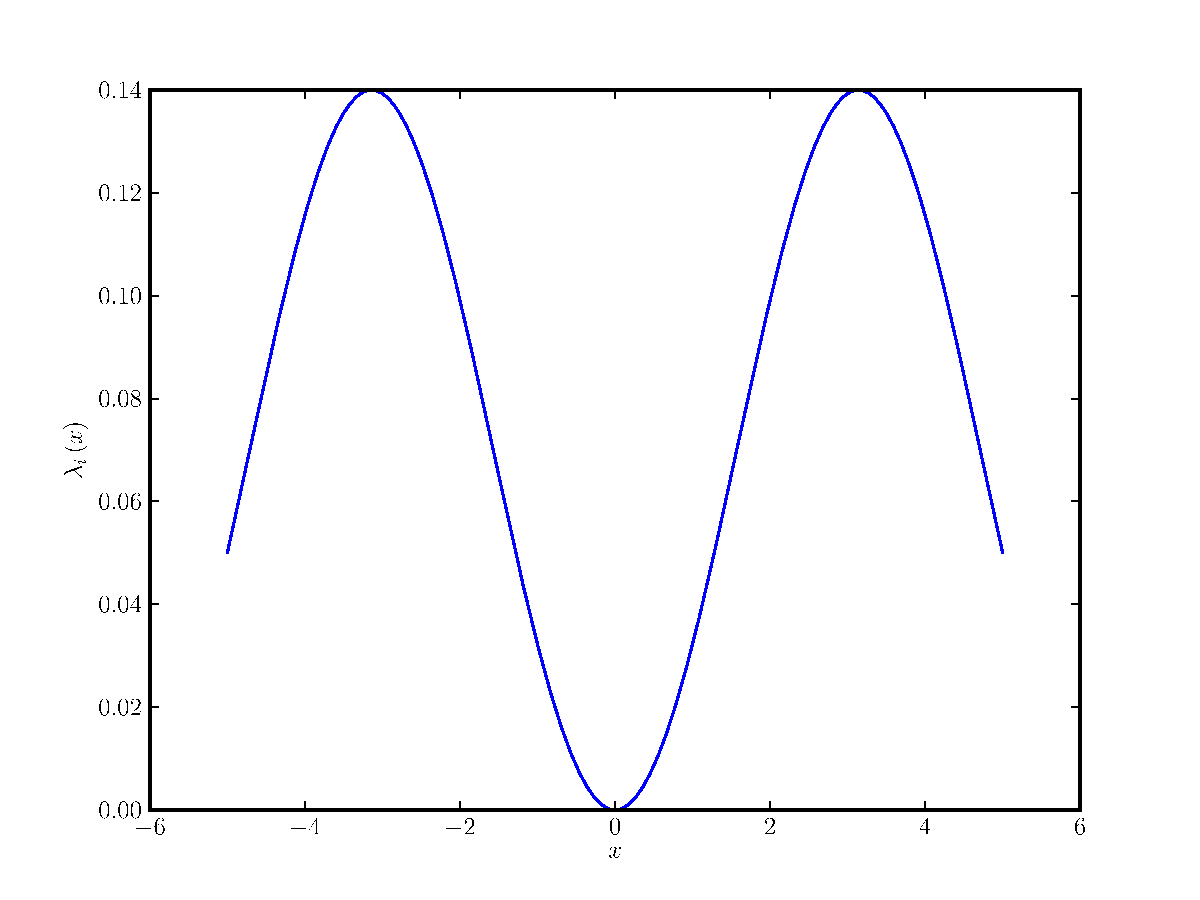
\includegraphics[scale=0.25]{./fig/cos_waves.pdf}
  \end{center}
\end{minipage}


\begin{minipage}{0.5\linewidth}
  Name:    \texttt{double\_well}
  \begin{equation*}
    V\ofs{x} = \left(\begin{smallmatrix}\sigma \left(1 - x^{2}\right)^{2}\end{smallmatrix}\right)
  \end{equation*}
  Defaults:
  \begin{align*}
    \sigma & = 1.0
  \end{align*}
\end{minipage}
\begin{minipage}{0.5\linewidth}
  \begin{center}
    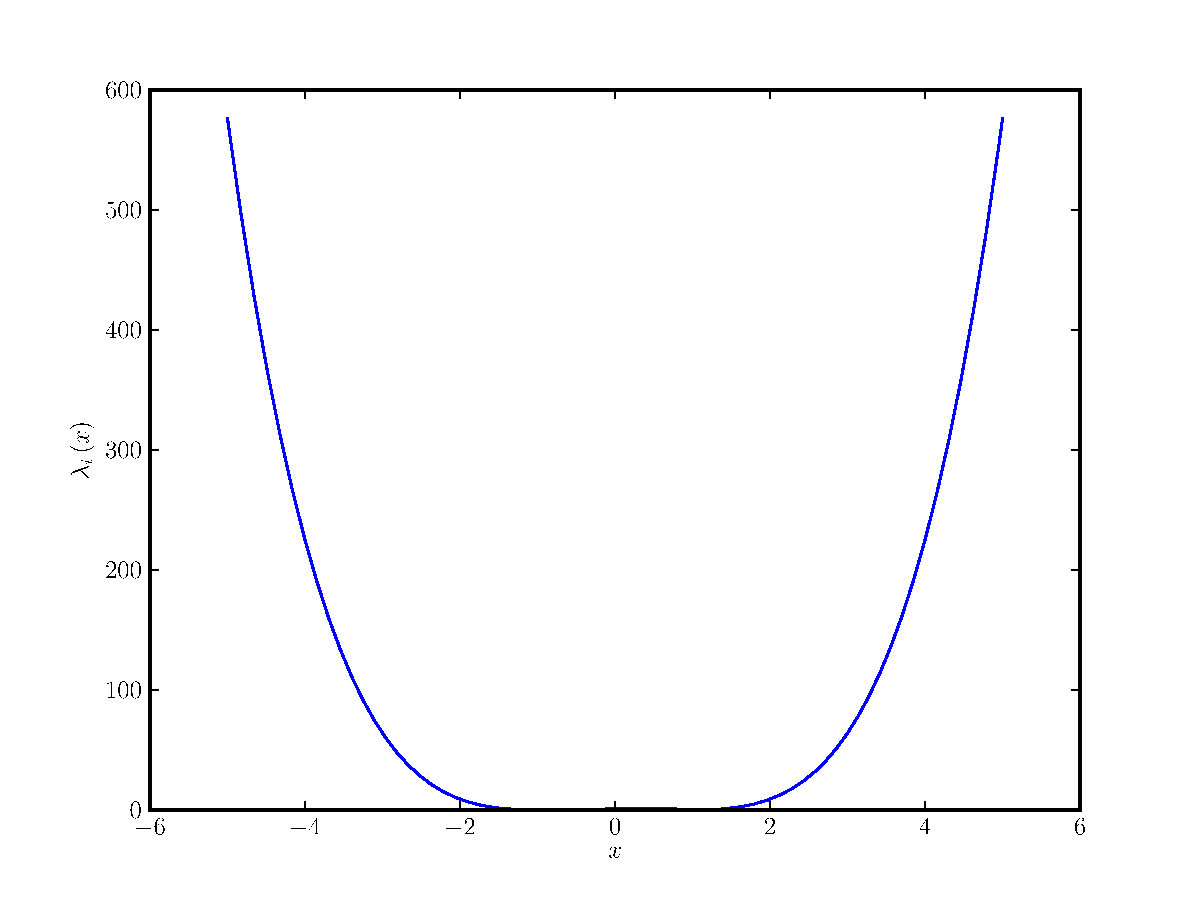
\includegraphics[scale=0.25]{./fig/double_well.pdf}
  \end{center}
\end{minipage}


\begin{minipage}{0.5\linewidth}
  Name:    \texttt{eckart}
  \begin{equation*}
    V\ofs{x} = \left(\begin{smallmatrix}\frac{\sigma}{\operatorname{cosh}^{2}\left(\frac{x}{a}\right)}\end{smallmatrix}\right)
  \end{equation*}
  Defaults:
  \begin{align*}
    \sigma & = 100 \cdot 3.8088 \cdot 10^{-4} \\
    a &= \frac{1.0}{2.0 \cdot 0.52918}
  \end{align*}
\end{minipage}
\begin{minipage}{0.5\linewidth}
  \begin{center}
    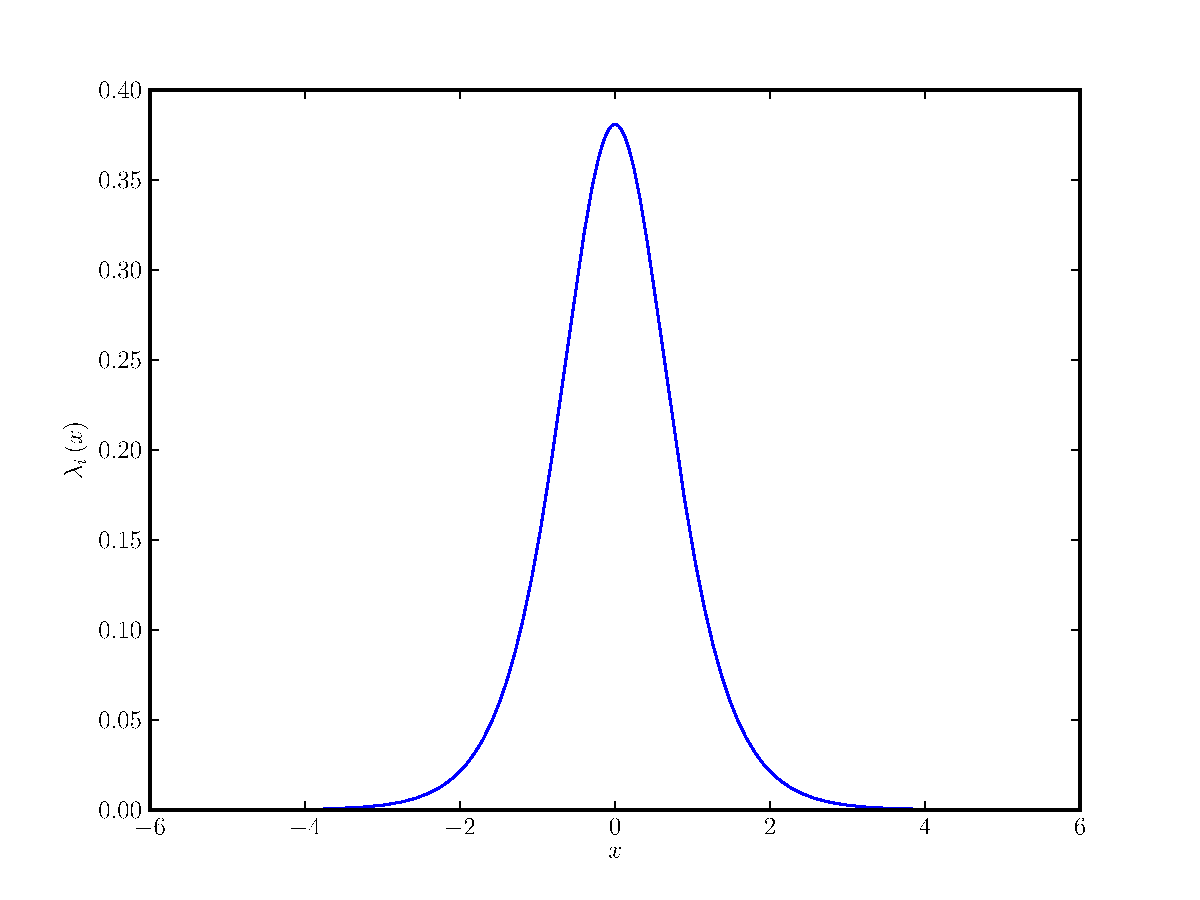
\includegraphics[scale=0.25]{./fig/eckart.pdf}
  \end{center}
\end{minipage}


\begin{minipage}{0.5\linewidth}
  Name:    \texttt{pert\_quadratic}
  \begin{equation*}
    V\ofs{x} = \left(\begin{smallmatrix}\frac{1}{2} \sigma x^{2} + \frac{1}{2} eps^{2} x^{2}\end{smallmatrix}\right)
  \end{equation*}
  Defaults:
  \begin{align*}
    \sigma & = 0.05
  \end{align*}
\end{minipage}
\begin{minipage}{0.5\linewidth}
  \begin{center}
    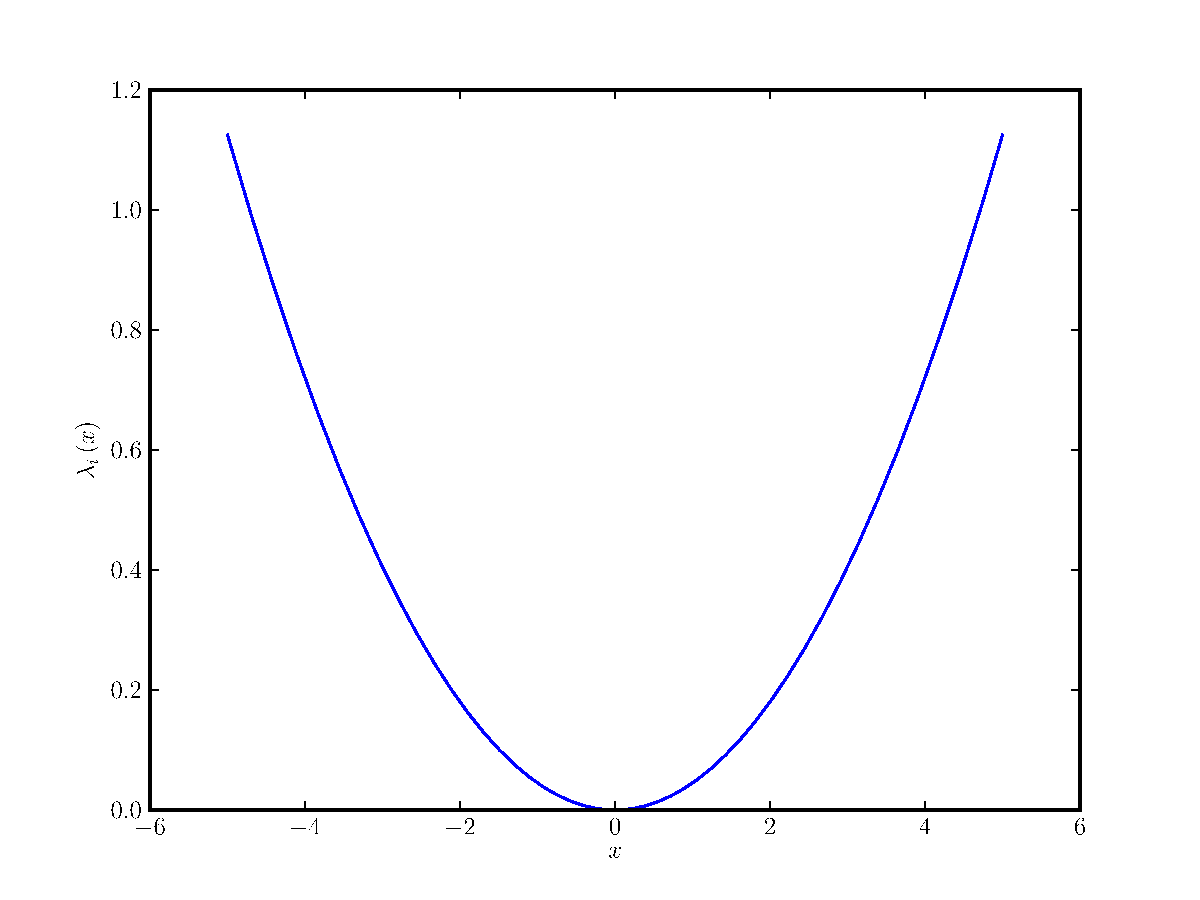
\includegraphics[scale=0.25]{./fig/pert_quadratic.pdf}
  \end{center}
\end{minipage}


\begin{minipage}{0.5\linewidth}
  Name:    \texttt{quadratic}
  \begin{equation*}
    V\ofs{x} = \left(\begin{smallmatrix}\frac{1}{2} \sigma x^{2}\end{smallmatrix}\right)
  \end{equation*}
  Defaults:
  \begin{align*}
    \sigma & = 0.5
  \end{align*}
\end{minipage}
\begin{minipage}{0.5\linewidth}
  \begin{center}
    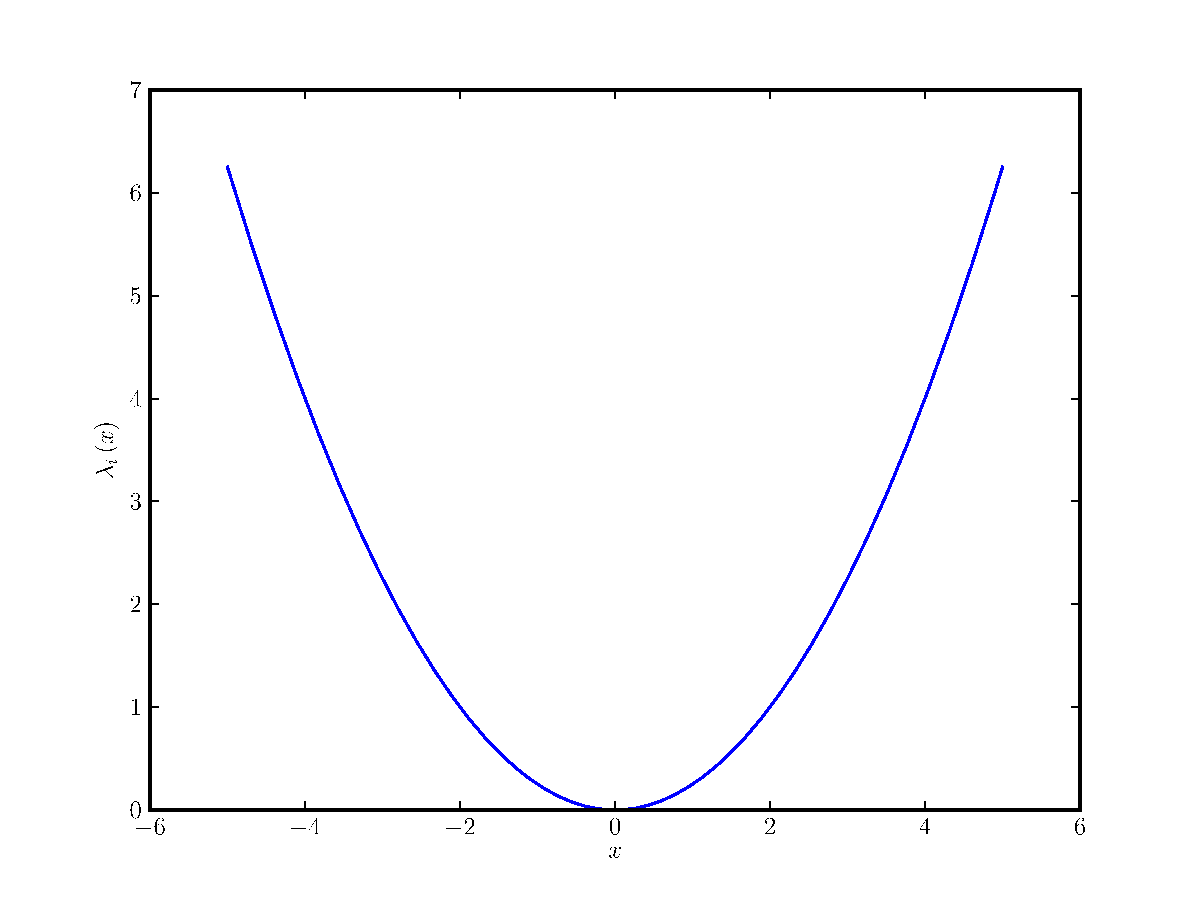
\includegraphics[scale=0.25]{./fig/quadratic.pdf}
  \end{center}
\end{minipage}


\begin{minipage}{0.5\linewidth}
  Name:    \texttt{quartic}
  \begin{equation*}
    V\ofs{x} = \left(\begin{smallmatrix}\frac{1}{4} \sigma x^{4}\end{smallmatrix}\right)
  \end{equation*}
  Defaults:
  \begin{align*}
    \sigma & = 0.05
  \end{align*}
\end{minipage}
\begin{minipage}{0.5\linewidth}
  \begin{center}
    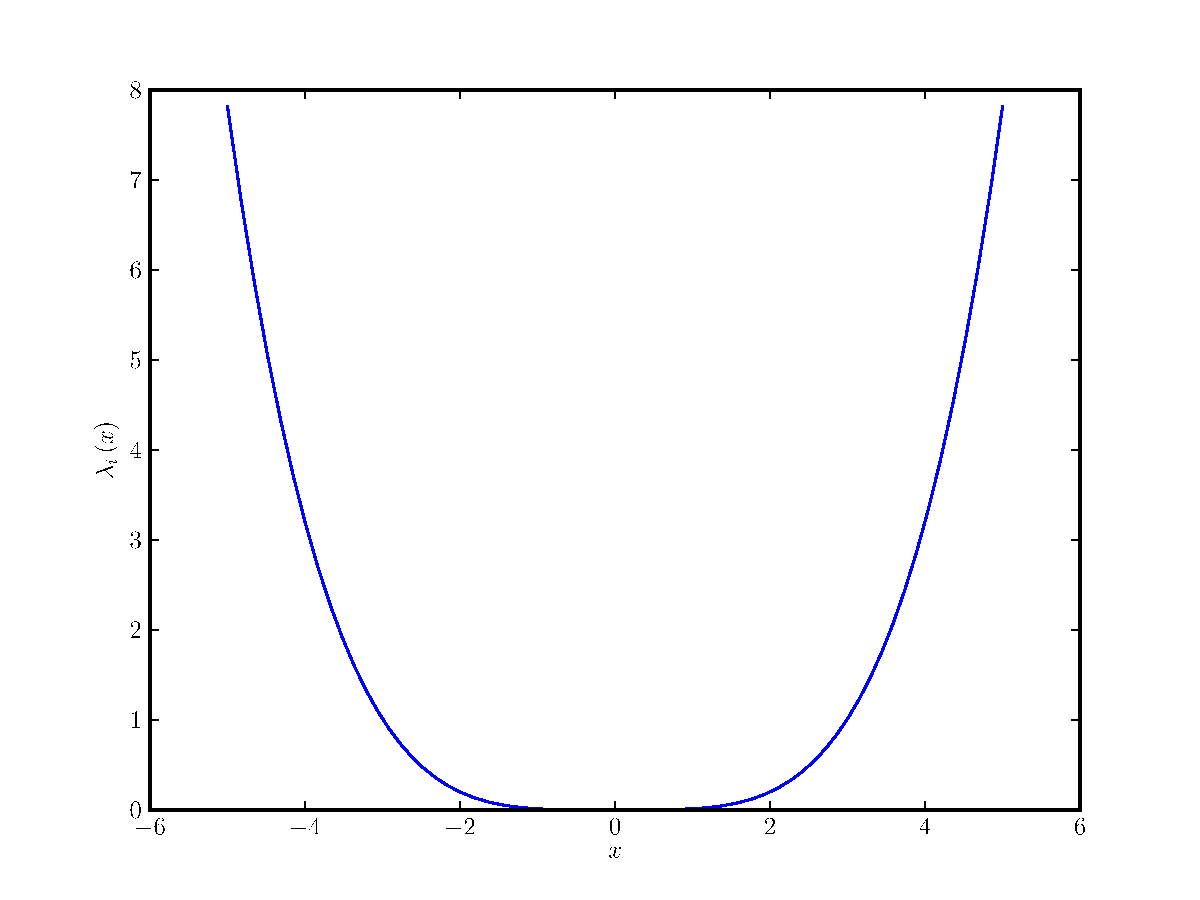
\includegraphics[scale=0.25]{./fig/quartic.pdf}
  \end{center}
\end{minipage}


\begin{minipage}{0.5\linewidth}
  Name:    \texttt{v\_shape}
  \begin{equation*}
    V\ofs{x} = \left(\begin{smallmatrix}\frac{1}{2} \sqrt{\operatorname{tanh}^{2}\left(x\right) + \frac{9}{16} eps^{2}}\end{smallmatrix}\right)
  \end{equation*}
\end{minipage}
\begin{minipage}{0.5\linewidth}
  \begin{center}
    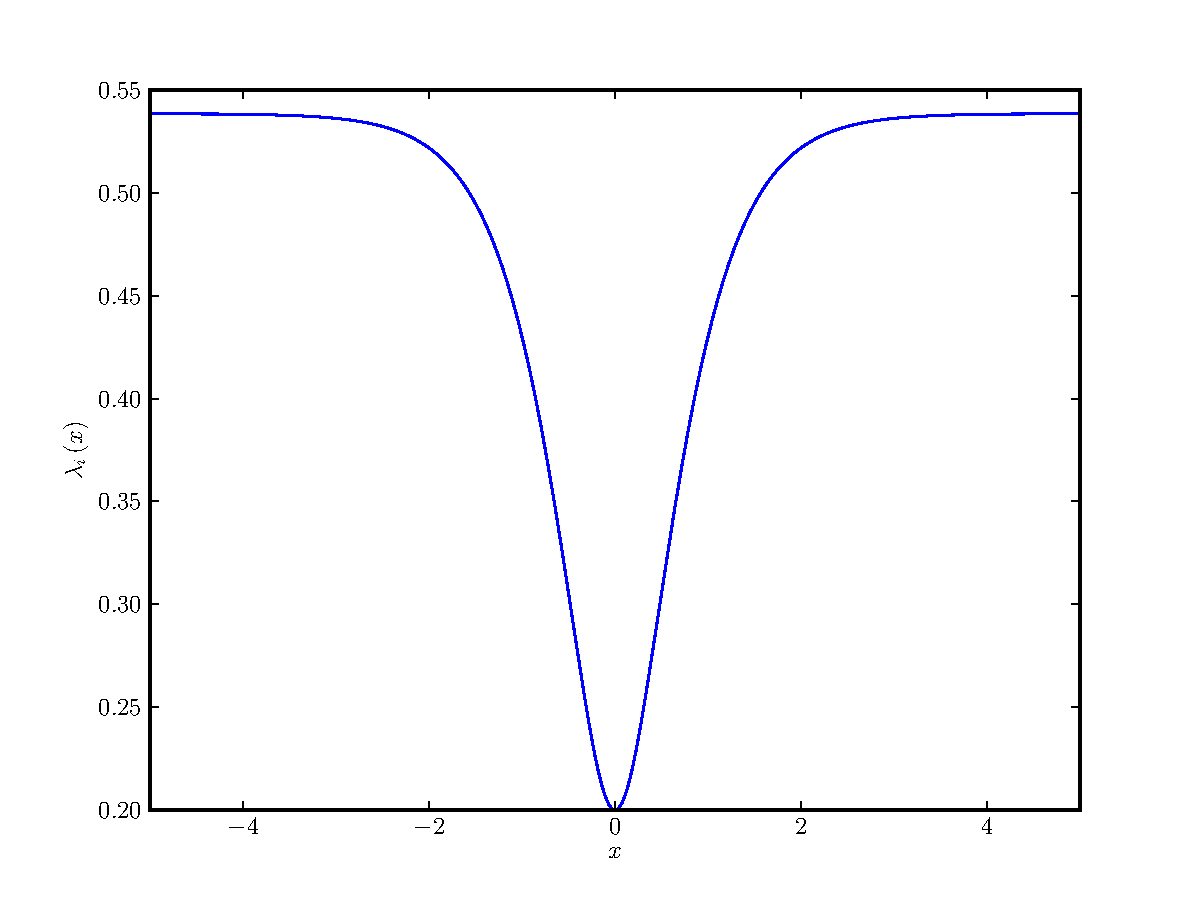
\includegraphics[scale=0.25]{./fig/v_shape.pdf}
  \end{center}
\end{minipage}


\begin{minipage}{0.5\linewidth}
  Name:    \texttt{wall}
  \begin{equation*}
    V\ofs{x} = \left(\begin{smallmatrix}\frac{1}{2} \pi + \operatorname{atan}\left(\sigma x\right)\end{smallmatrix}\right)
  \end{equation*}
  Defaults:
  \begin{align*}
    \sigma & = 10.0
  \end{align*}
\end{minipage}
\begin{minipage}{0.5\linewidth}
  \begin{center}
    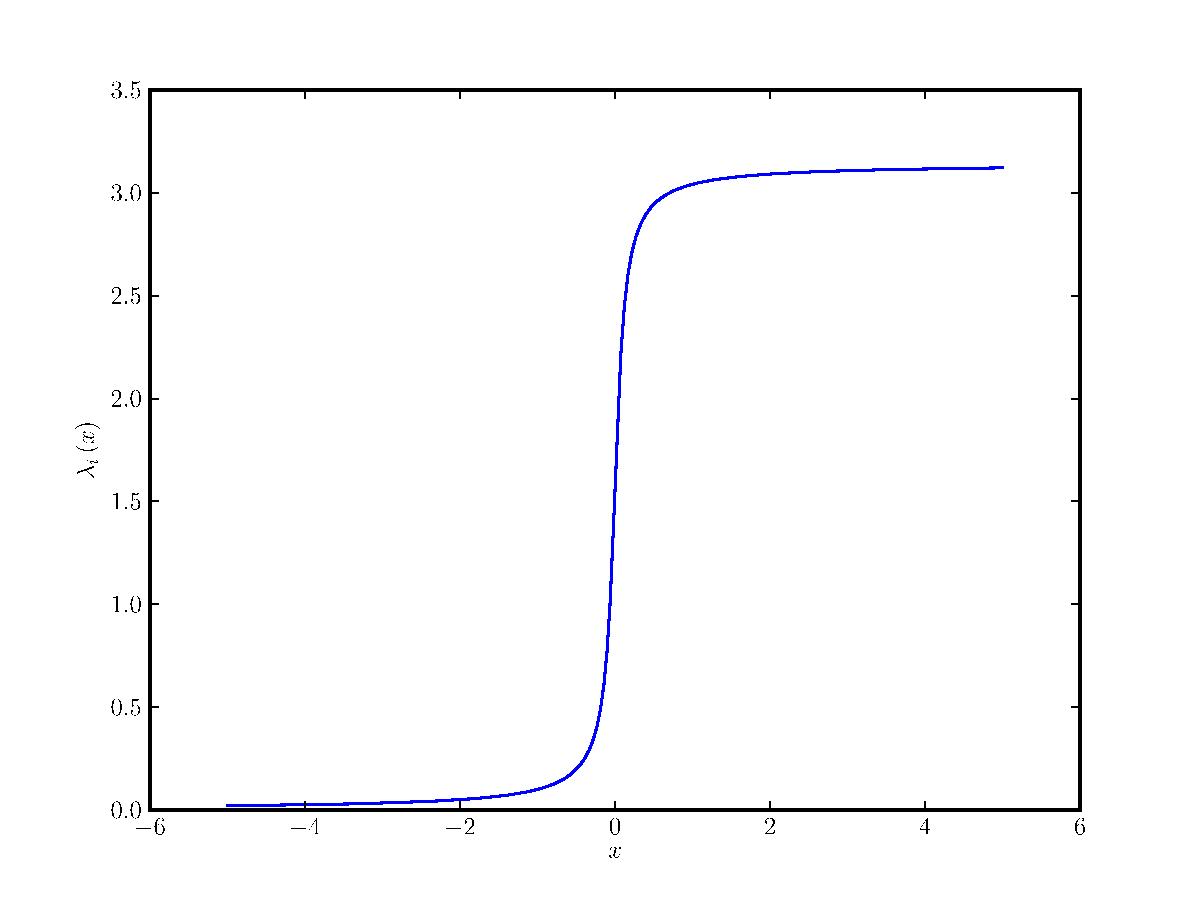
\includegraphics[scale=0.25]{./fig/wall.pdf}
  \end{center}
\end{minipage}


\subsubsection{Potentials with two energy levels}


\begin{minipage}{0.5\linewidth}
  Name:    \texttt{delta\_gap}
  \begin{equation*}
    V\ofs{x} = \left(\begin{smallmatrix}\frac{1}{2} \operatorname{tanh}\left(x\right) & \delta\\\delta & - \frac{1}{2} \operatorname{tanh}\left(x\right)\end{smallmatrix}\right)
  \end{equation*}
\end{minipage}
\begin{minipage}{0.5\linewidth}
  \begin{center}
    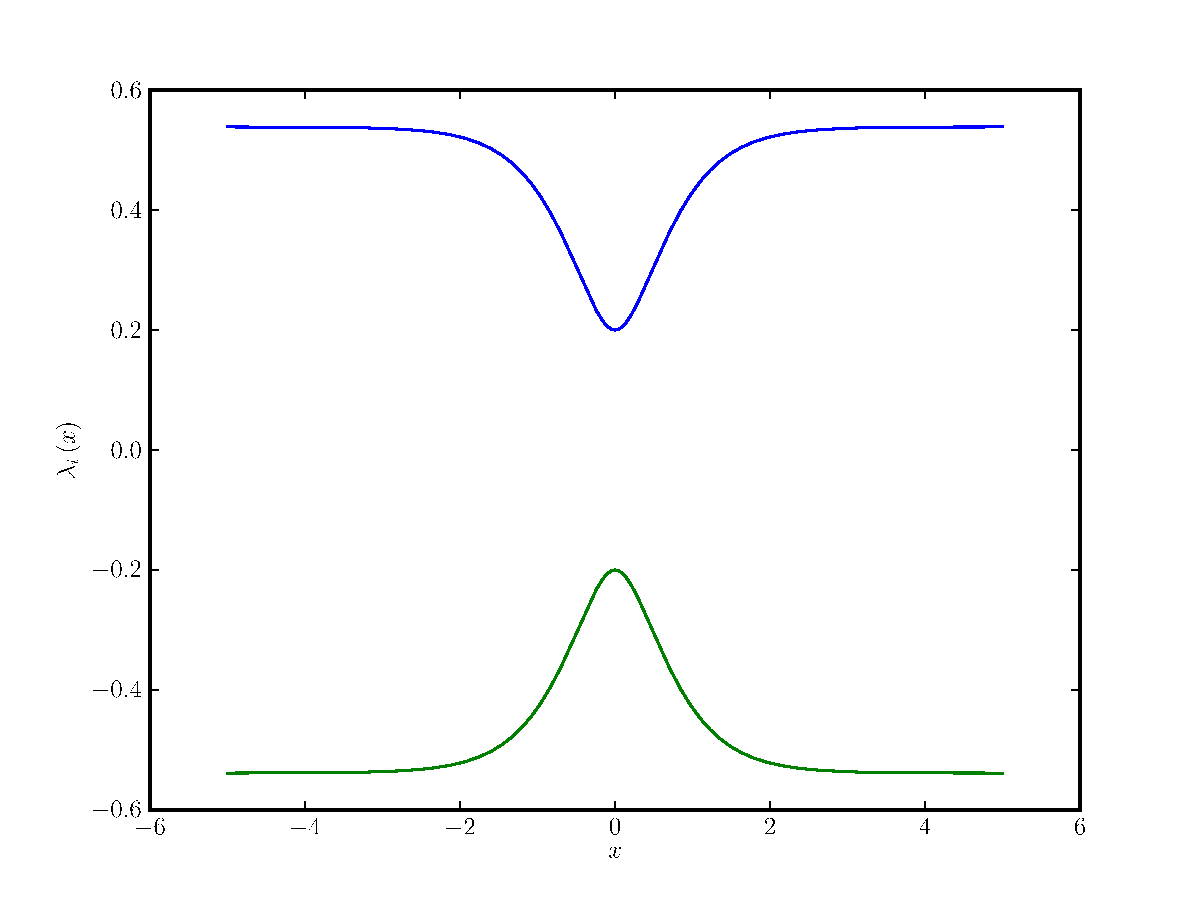
\includegraphics[scale=0.25]{./fig/delta_gap.pdf}
  \end{center}
\end{minipage}


\begin{minipage}{0.5\linewidth}
  Name:    \texttt{delta\_gap\_diag}
  \begin{equation*}
    V\ofs{x} = \left(\begin{smallmatrix}\sqrt{\delta^{2} + \frac{1}{4} \operatorname{tanh}^{2}\left(x\right)} & 0\\0 & - \sqrt{\delta^{2} + \frac{1}{4} \operatorname{tanh}^{2}\left(x\right)}\end{smallmatrix}\right)
  \end{equation*}
\end{minipage}
\begin{minipage}{0.5\linewidth}
  \begin{center}
    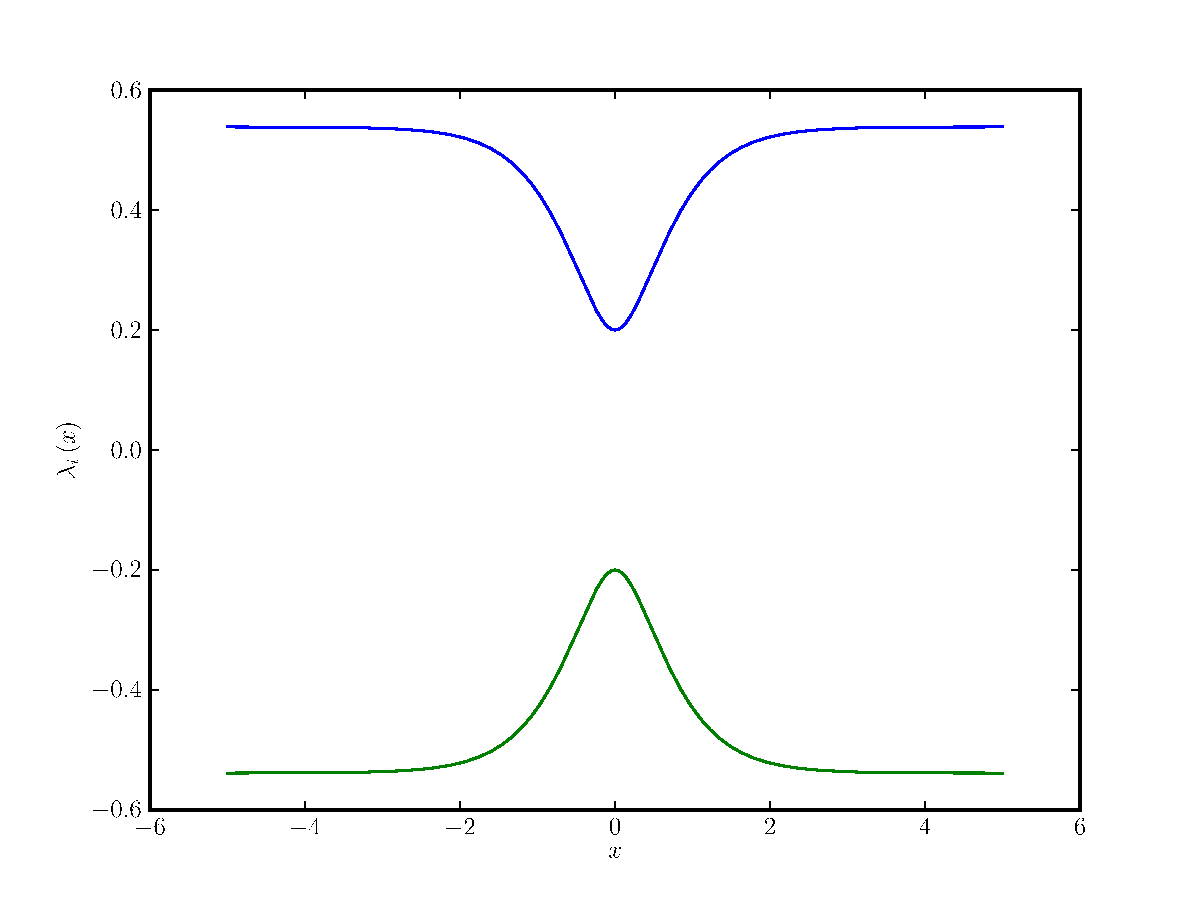
\includegraphics[scale=0.25]{./fig/delta_gap_diag.pdf}
  \end{center}
\end{minipage}


\begin{minipage}{0.75\linewidth}
  Name:    \texttt{two\_crossings}
  \begin{equation*}
    V\ofs{x} = \left(\begin{smallmatrix}\operatorname{tanh}\left(\rho + x\right) \operatorname{tanh}\left(x - \rho\right) & \delta\\\delta & - \operatorname{tanh}\left(\rho + x\right) \operatorname{tanh}\left(x - \rho\right)\end{smallmatrix}\right)
  \end{equation*}
  Defaults:
  \begin{align*}
    \rho & = 3.0
  \end{align*}
\end{minipage}
\begin{minipage}{0.25\linewidth}
  \begin{center}
    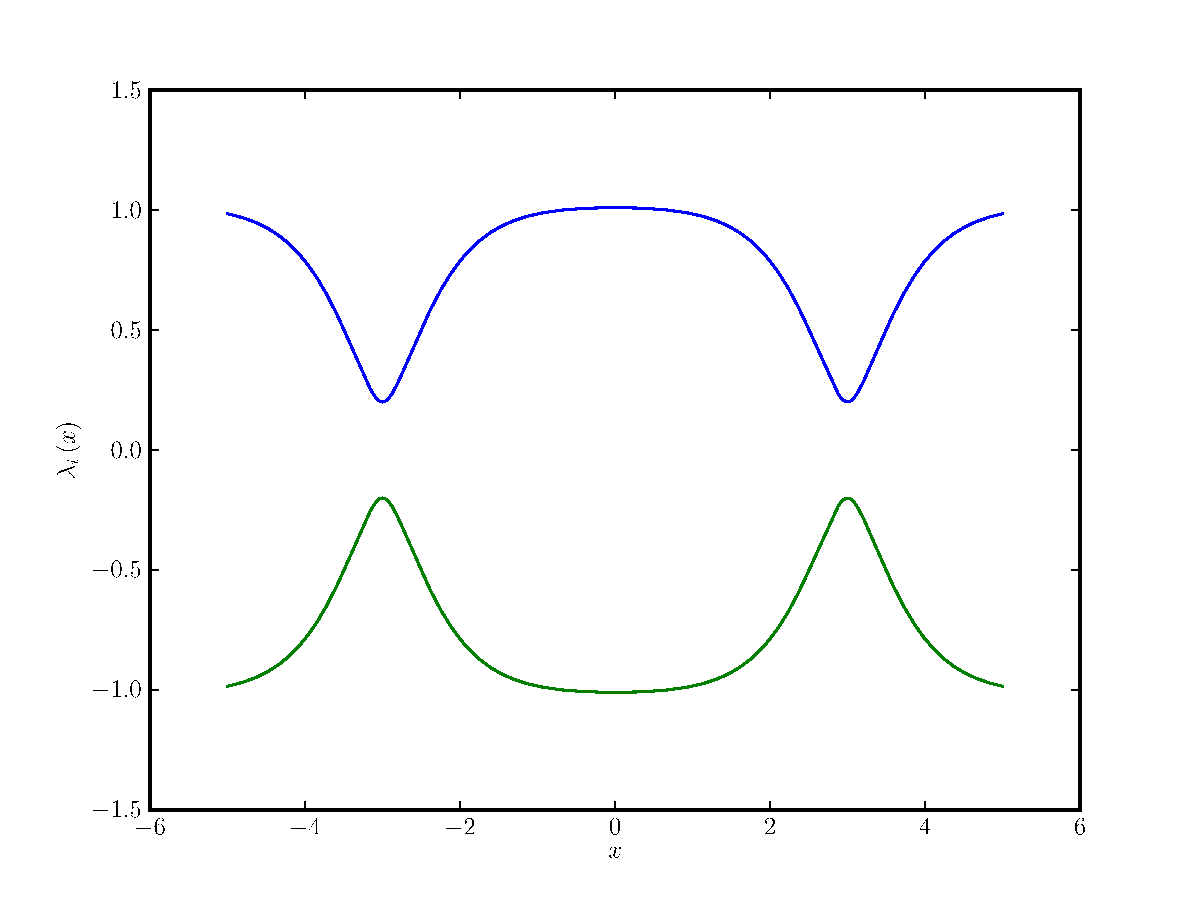
\includegraphics[scale=0.25]{./fig/two_crossings.pdf}
  \end{center}
\end{minipage}


\begin{minipage}{0.5\linewidth}
  Name:    \texttt{two\_quadratic}
  \begin{equation*}
    V\ofs{x} = \left(\begin{smallmatrix}\frac{1}{2} \sigma x^{2} & 0\\0 & \frac{1}{2} \sigma x^{2}\end{smallmatrix}\right)
  \end{equation*}
  Defaults:
  \begin{align*}
    \sigma & = 0.05
  \end{align*}
\end{minipage}
\begin{minipage}{0.5\linewidth}
  \begin{center}
    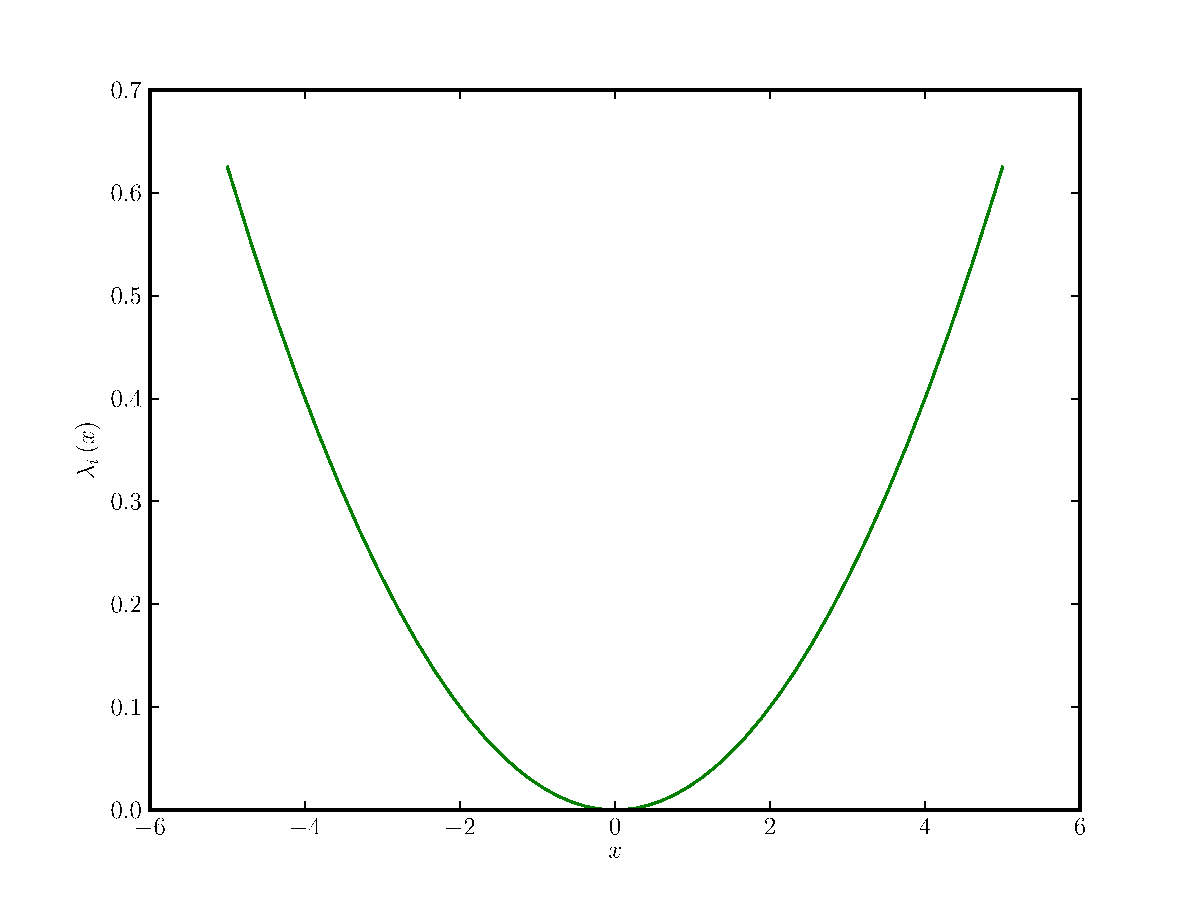
\includegraphics[scale=0.25]{./fig/two_quadratic.pdf}
  \end{center}
\end{minipage}


\begin{minipage}{0.5\linewidth}
  Name:    \texttt{two\_quartic}
  \begin{equation*}
    V\ofs{x} = \left(\begin{smallmatrix}\frac{1}{4} \sigma x^{4} & 0\\0 & \frac{1}{8} \sigma x^{4}\end{smallmatrix}\right)
  \end{equation*}
  Defaults:
  \begin{align*}
    \sigma & = 1.0
  \end{align*}
\end{minipage}
\begin{minipage}{0.5\linewidth}
  \begin{center}
    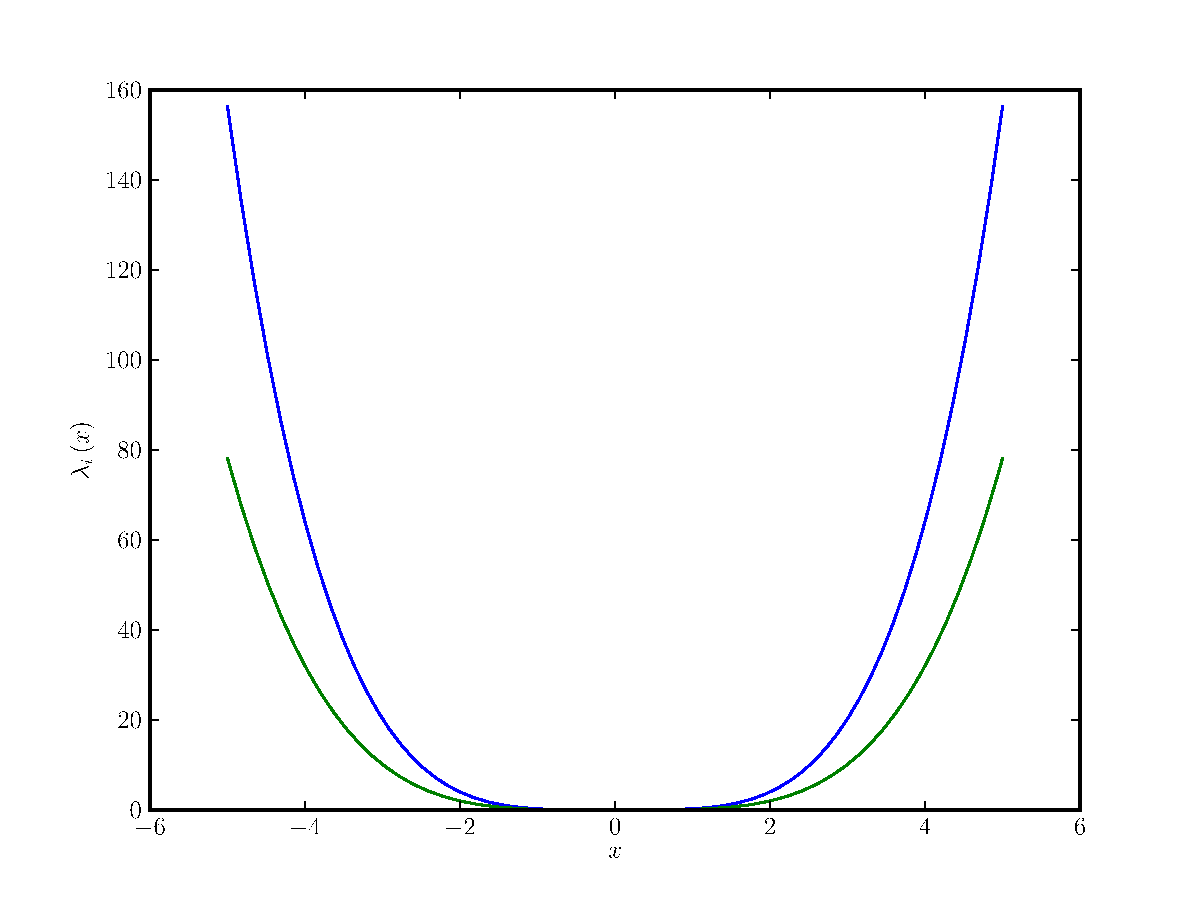
\includegraphics[scale=0.25]{./fig/two_quartic.pdf}
  \end{center}
\end{minipage}


\subsubsection{Potentials with three energy levels}


\begin{minipage}{0.75\linewidth}
  Name:    \texttt{three\_levels}
  \begin{equation*}
    V\ofs{x} = \left(\begin{smallmatrix}\operatorname{tanh}\left(\rho + x\right) + \operatorname{tanh}\left(x - \rho\right) & \delta_{1} & \delta_{2}\\\delta_{1} & - \operatorname{tanh}\left(\rho + x\right) & 0\\\delta_{2} & 0 & 1 - \operatorname{tanh}\left(x - \rho\right)\end{smallmatrix}\right)
  \end{equation*}
  Defaults:
  \begin{align*}
    \rho & = 3.0
  \end{align*}
\end{minipage}
\begin{minipage}{0.25\linewidth}
  \begin{center}
    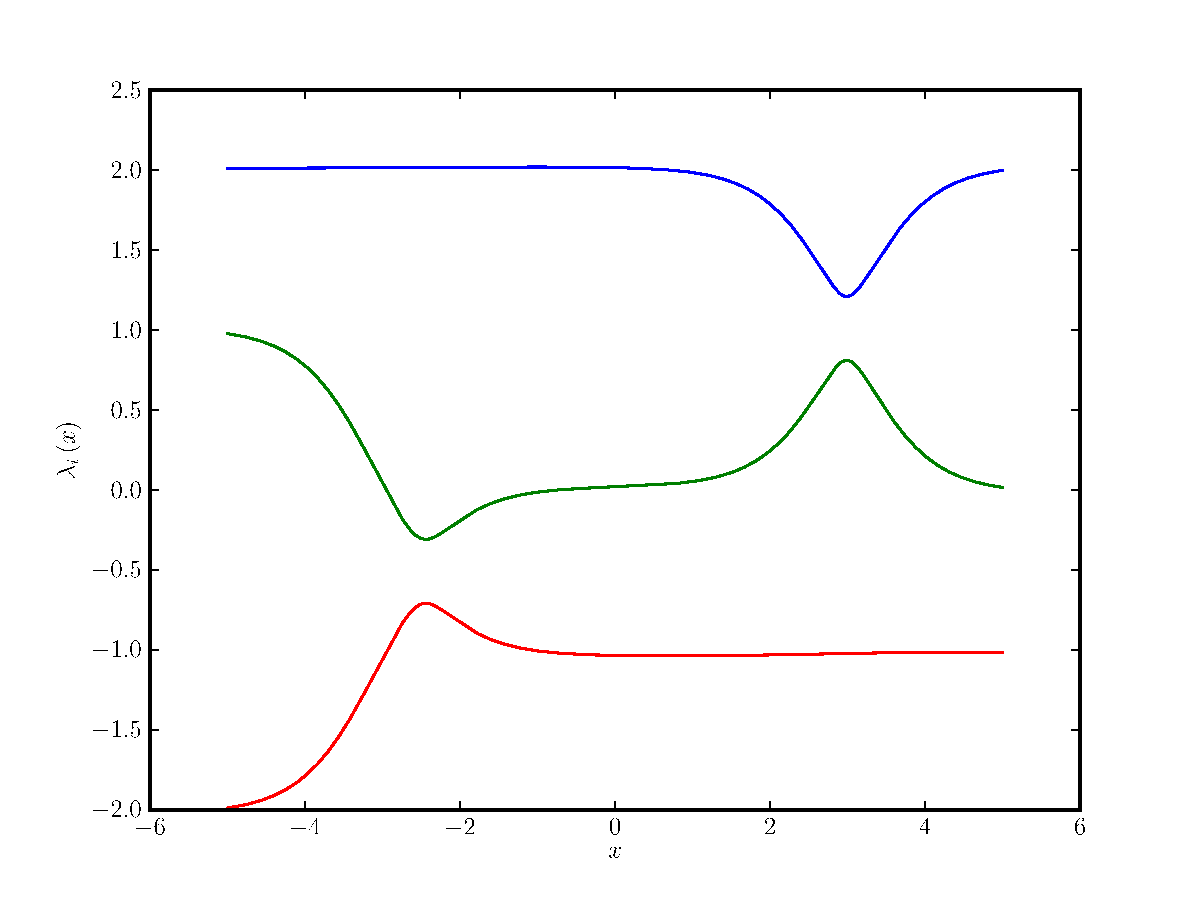
\includegraphics[scale=0.25]{./fig/three_levels.pdf}
  \end{center}
\end{minipage}


\begin{minipage}{0.5\linewidth}
  Name:    \texttt{three\_quadratic}
  \begin{equation*}
    V\ofs{x} = \left(\begin{smallmatrix}\frac{1}{2} \sigma x^{2} & 0 & 0\\0 & \frac{1}{2} \sigma x^{2} & 0\\0 & 0 & \frac{1}{2} \sigma x^{2}\end{smallmatrix}\right)
  \end{equation*}
  Defaults:
  \begin{align*}
    \sigma & = 0.05
  \end{align*}
\end{minipage}
\begin{minipage}{0.5\linewidth}
  \begin{center}
    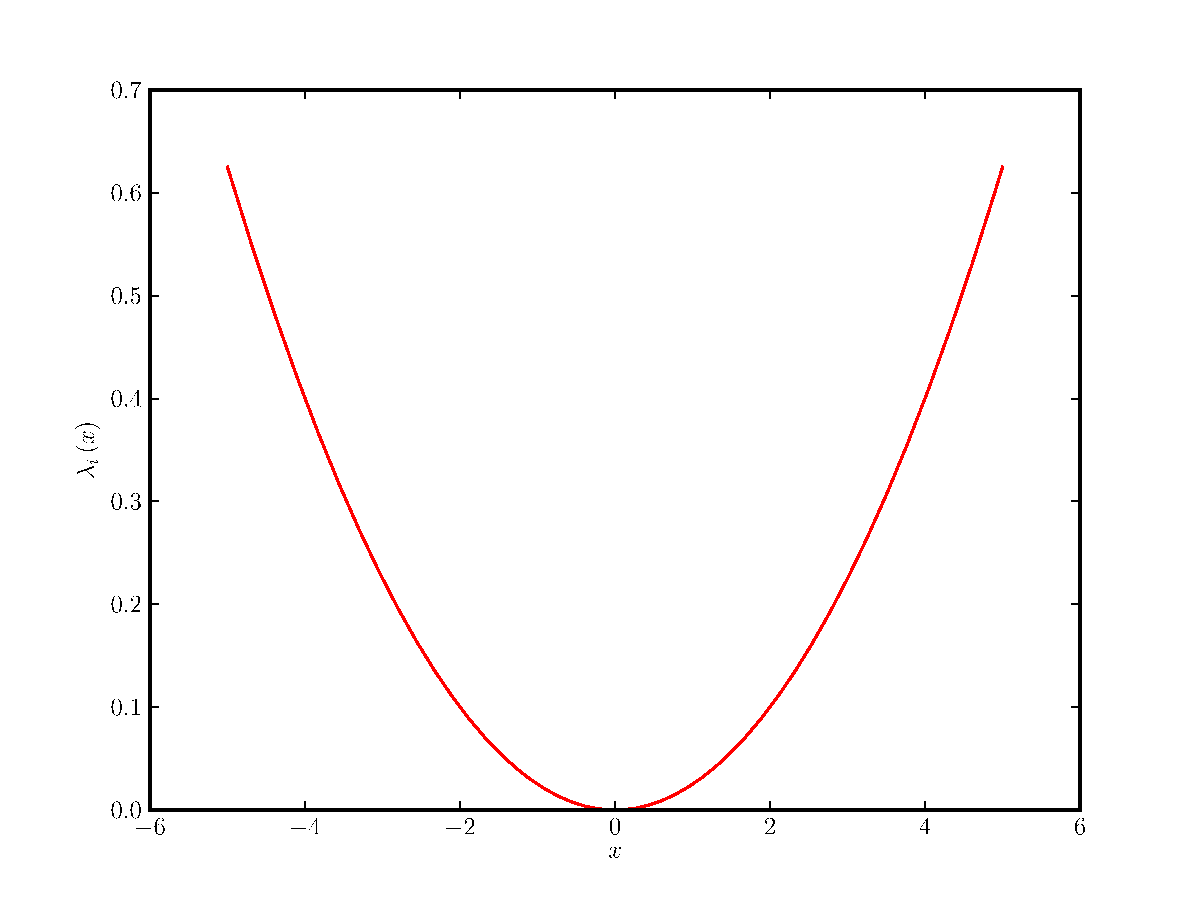
\includegraphics[scale=0.25]{./fig/three_quadratic.pdf}
  \end{center}
\end{minipage}


\subsubsection{Potentials with four energy levels}


\begin{minipage}{0.5\linewidth}
  Name:    \texttt{four\_powers}
  \begin{equation*}
    V\ofs{x} = \left(\begin{smallmatrix}\frac{1}{2} \sigma x^{2} & 0 & 0 & 0\\0 & \frac{1}{4} \sigma x^{4} & 0 & 0\\0 & 0 & \frac{1}{6} \sigma x^{6} & 0\\0 & 0 & 0 & \frac{1}{8} \sigma x^{8}\end{smallmatrix}\right)
  \end{equation*}
  Defaults:
  \begin{align*}
    \sigma & = 0.05
  \end{align*}
\end{minipage}
\begin{minipage}{0.5\linewidth}
  \begin{center}
    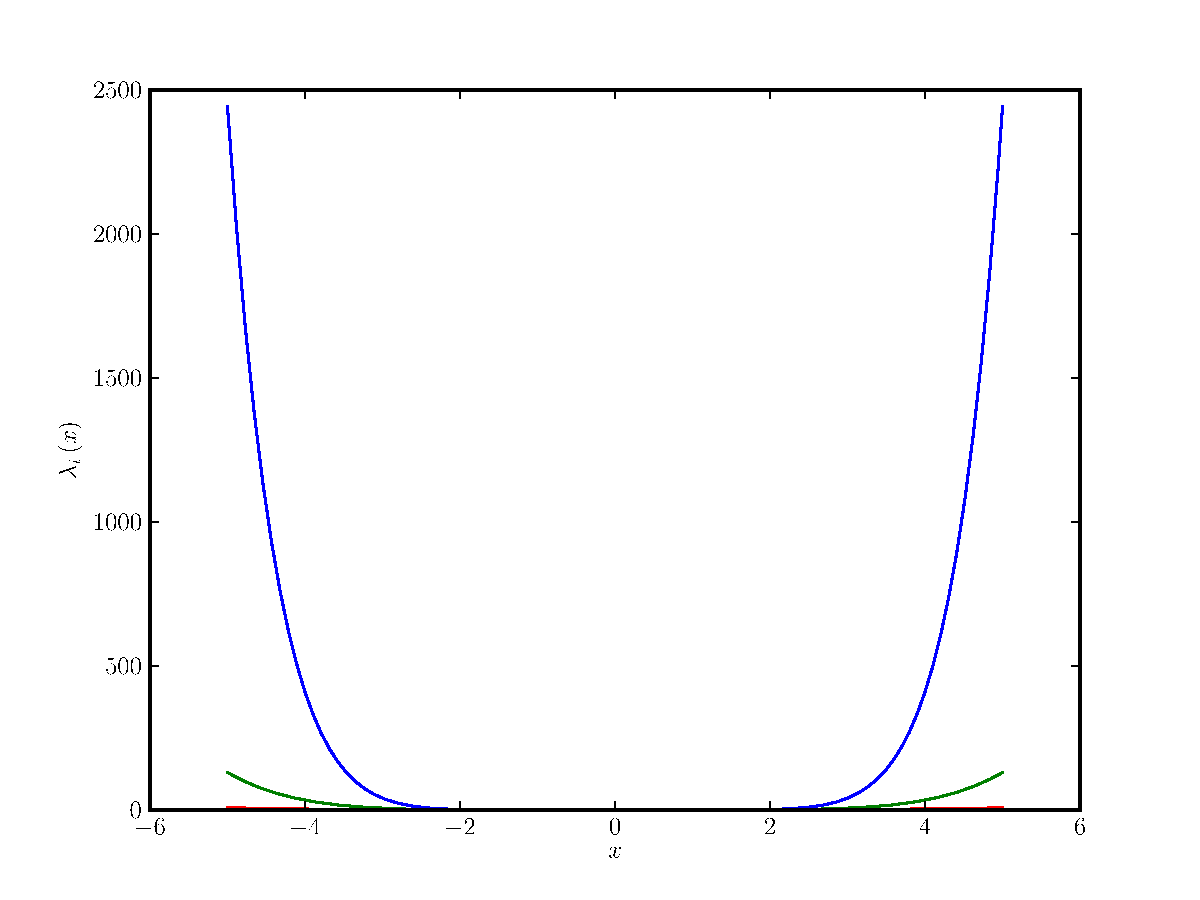
\includegraphics[scale=0.25]{./fig/four_powers.pdf}
  \end{center}
\end{minipage}


\subsubsection{Potentials with five energy levels}


\begin{minipage}{0.5\linewidth}
  Name:    \texttt{five\_quadratic}
  \begin{equation*}
    V\ofs{x} = \left(\begin{smallmatrix}\frac{1}{2} \sigma x^{2} & 0 & 0 & 0 & 0\\0 & \frac{1}{2} \sigma x^{2} & 0 & 0 & 0\\0 & 0 & \frac{1}{2} \sigma x^{2} & 0 & 0\\0 & 0 & 0 & \frac{1}{2} \sigma x^{2} & 0\\0 & 0 & 0 & 0 & \frac{1}{2} \sigma x^{2}\end{smallmatrix}\right)
  \end{equation*}
  Defaults:
  \begin{align*}
    \sigma & = 0.05
  \end{align*}
\end{minipage}
\begin{minipage}{0.5\linewidth}
  \begin{center}
    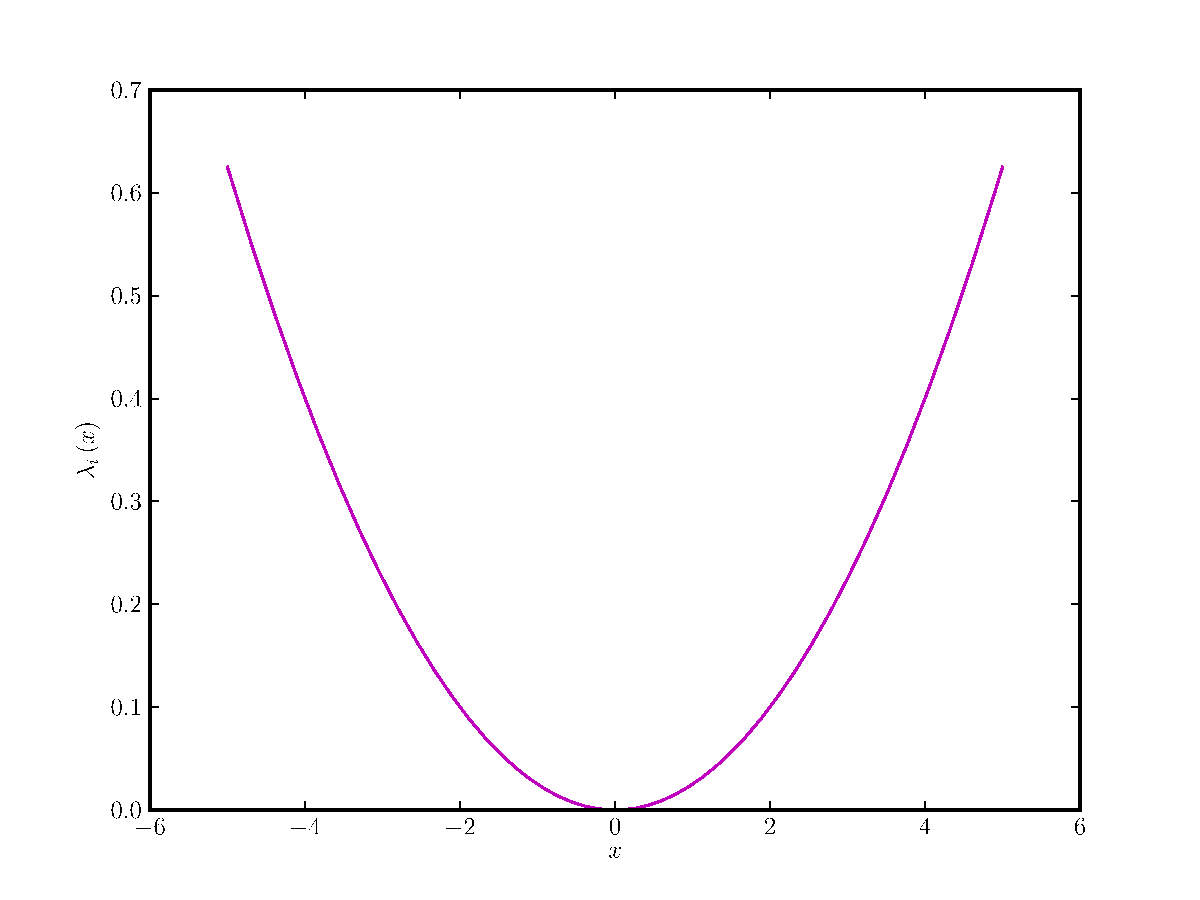
\includegraphics[scale=0.25]{./fig/five_quadratic.pdf}
  \end{center}
\end{minipage}


\subsection{Time propagation algorithms}

At the moment, three algorithms for time propagation of initial values are
implemented.

\begin{center}
\begin{tabular}{ll}
  Name & Description \\
  \hline
  \texttt{fourier} & Fourier propagation / Operator splitting \\
  \texttt{hagedorn} & Homogeneous Hagedorn wavepackets \\
  \texttt{multihagedorn} & Inhomogeneous Hagedorn wavepackets \\
%   \texttt{spawn} & Spawning propagation for tunneling problems
\end{tabular}
\end{center}


\subsection{Specifying initial values}

Initial values are always specified as wavepackets. For the Fourier propagator,
the packets are sampled at the grid nodes and for packet based algorithms, these
initial packets are just propagated. The two configuration variables \texttt{parameters}
and \texttt{coefficients} are responsible for specifying the initial wavepackets.
Their values are interpreted as usual but let's look at this important part
a bit closer.

\subsubsection{For the \texttt{fourier} Propagator}

The initial values for the \texttt{fourier} propagator are given in the simulation
configuration file by the variable \texttt{initial\_values}. The data format is
a list of arbitrary length. Each entry is a list itself having the format:

\begin{verbatim}
  [ level, parameters, [(index,value), (index,value), ...] ]
\end{verbatim}

where the \texttt{level} is the energy level, the \texttt{parameters} is a 5-tuple
of the usual form \texttt{(P,Q,S,p,q)} containing the wavepacket's parameter. The
third part is a list containing one or several \texttt{(index,value)} pairs
which hold the value $c_i$ of the coefficient with index $i$. We know that
this is all the data necessary for constructing a wavepacket that lives on
the given energy level. (But remember that these packets are sampled at the grid
nodes later to be usable for the Fourier propagation.)

This input format allows us to place several wavepackets on the same energy level,
for example the following valid specification places two Gaussian packets
which will run into each other and bounce off:

\begin{verbatim}
  initial_values = [[ 0, (P, Q, S, -0.5,  2.0), [(0,1.0)]],
                    [ 0, (P, Q, S,  0.5, -2.0), [(0,1.0)]]]
\end{verbatim}

For compatibility reasons the input can also be of the format described
in the next two sections. This allows for sharing of simulation configurations.

\subsubsection{For the \texttt{hagedorn} Propagator}

For this propagator we need one set of parameters which belong to
the leading component. With these parameters we then set up a homogeneous
wavepacket. We can specify the parameters as follows:

\begin{verbatim}
  parameters = (P, Q, S, p, q)
\end{verbatim}

with some meaningful values for $Q$, $P$, $S$ and $q$ and $p$. For compatibility
with the inhomogeneous case, we can also specify the parameters as:

\begin{verbatim}
  parameters = [ (P0, Q0, S0, p0, q0), ..., (Pn, Qn, Sn, pn, qn) ]
\end{verbatim}

where there are as many inner tuples as energy levels. The initialisation
code then picks just the single tuple with its index matching the
\texttt{leading\_component} value. This allows easy sharing of
configuration files with minimal editing.

The coefficients $c_i$ of the linear combination are specified for each
level separately. There is a list of \texttt{(index,value)} pairs for
each energy level and all these lists are collected in one big list
assigned to the variable \texttt{coefficients}. This could for example look like:

\begin{verbatim}
  coefficients = [[ (0,1.0), (2,0.5), (4,0.2)],
                  [ (0,0.1), (3,1.2)]]
\end{verbatim}

where we have two energy levels (note that the wave function here is not normalized!).
These \texttt{(index,value)} pairs give the value $c_i$ of the coefficient
with index $i$. For example the list containing only the pair \texttt{[ (2,1.0) ]}
yields a $\varphi_2$ packet while the list \texttt{[ (0,0.5), (1,0.5) ]} gives
a superposition of $\frac{1}{2} \left( \varphi_0 + \varphi_1 \right)$. If you
wish to have no wavepacket on an energy level just provide the dummy pair \texttt{[ (0,0.0) ]}.

\subsubsection{For the \texttt{multihagedorn} Propagator}

This propagator needs a set of parameters for each energy level. Thus
the data structure must look like:

\begin{verbatim}
  parameters = [ (P0, Q0, S0, p0, q0), ..., (Pn, Qn, Sn, pn, qn) ]
\end{verbatim}

where there are as many inner tuples as energy levels. The coefficients $c_i$
are specified the same way as in the homogeneous case above.


\subsection{Required parameter sets}

The simulations can be configured with a very flexible scheme. Namely is possible
to just specify the values that are really necessary and omit all others. There
are some input parameters that have to be provided in any case and many others that
are only necessary for a specific algorithm or are pure optional.

In this section of the manual all parameters that can be provided are listed.
But you are free to define additional parameters and use them in a data evaluation
script. Just make sure there is no variable name clash.

% \begin{description}
%   \item[\texttt{}]
%   \begin{itemize}
%     \item
%     \item
%   \end{itemize}
% \end{description}

\subsubsection{Parameters for all propagation algorithms}

\begin{description}
  \item[\texttt{algorithm}] The simulation algorithm
  \begin{itemize}
    \item Possible values: \texttt{fourier}, \texttt{hagedorn}, \texttt{multihagedorn}, \texttt{spawn}
    \item Data type: string
  \end{itemize}

  \item[\texttt{potential}] The potential
  \begin{itemize}
    \item Possible values: see section \ref{sec:ready_made_potentials}
    \item Data type: string or dict
  \end{itemize}

  \item[\texttt{T}] The time when the simulation stops
  \begin{itemize}
    \item Possible values: Non-negative float
    \item Data type: float
  \end{itemize}

  \item[\texttt{dt}] The size of a single time step
  \begin{itemize}
    \item Possible values: Non-negative float
    \item Data type: float
  \end{itemize}

  \item[\texttt{eps}] The semi-classical scaling parameter
  \begin{itemize}
    \item Possible values: Non-negative float
    \item Data type: float
  \end{itemize}

  \item[\texttt{parameters}] The Hagedorn parameters $\{P, Q, S, p, q \}$ of the
    initial wave packets. The exact format of this variable depends on the
    simulation algorithm used, see above.

  \item[\texttt{coefficients}] A list with the lists of (index,value) tuples that
    set the coefficients of the basis functions for the initial wavepackets. The
    exact format of this variable depends on the simulation algorithm used, see above.

  \item[\texttt{write\_nth}] Save simulation data every n-th timestep
  \begin{itemize}
    \item Possible values: Positive Integer where the case 0 is interpreted as
          \emph{never}. In this case only the initial values are saved.
    \item Data type: integer
    \item Default value: is 0 if no other value is provided.
  \end{itemize}

  \item[\texttt{save\_at}] A list of times and/or timesteps when saving of the
    simulation data takes place. (Which data are saved depends on the implementation
    of the respective \texttt{SimulationLoop} subclass.)
  \begin{itemize}
    \item Possible values: A list of integers and/or floats. Integers are interpreted
    as timesteps and floats as (absolute) times. Be always aware of this difference
    in interpretation!
    \item Data type: integer or float
    \item Default value: an empty list, thus saving at special points in time
    is not enabled.
  \end{itemize}

  \item[\texttt{matrix\_exponential}] Choose the algorithm used for computing the matrix exponential.
  \begin{itemize}
    \item Possible values: \texttt{"pade"}, \texttt{"arnoldi"}
    \item Data type: string
    \item Default value: \texttt{"pade"}
  \end{itemize}

  \item[\texttt{arnoldi\_steps}] The number of arnoldi steps performed. Use this together with
  the parameter \texttt{matrix\_exponential} set to \texttt{"arnoldi"}.
  \begin{itemize}
    \item Possible values: positive integers
    \item Data type: integer
    \item Default value: 20
  \end{itemize}
\end{description}

\subsubsection{Parameters for the \texttt{fourier} propagator}

\begin{description}

  \item[\texttt{initial\_values}] A specific input format for the initial values.
    This allows to place an arbitrary number of wavepackets on any energy level.
    A valid configuration must either have this variable set or both of
    \texttt{parameters} and \texttt{coefficients}. If all three are given, this
    takes precedence.

  \item[\texttt{ngn}] The number of grid nodes used for the Fourier transformation.
  \begin{itemize}
    \item Possible values: Integer, optimal is a power of 2 but this is not necessary.
    \item Data type: integer
  \end{itemize}

  \item[\texttt{f}] A scalar number that determines the extension of the computational domain.
  \begin{itemize}
    \item Possible values: A non-negative float
    \item Data type: float
  \end{itemize}
\end{description}

Note: You must specify a \texttt{basis\_size} (see below) for the Fourier propagator too
because we compute initial values from wavepackets.

\subsubsection{Parameters for the \texttt{hagedorn} propagator}

\begin{description}
  \item[\texttt{basis\_size}] Number of basis functions used for homogeneous Hagedorn wavepackets.
  \begin{itemize}
    \item Possible values: Non-negative integer larger than $2$.
    \item Data type: integer
  \end{itemize}

  \item[\texttt{leading\_component}] The leading component is the eigenvalue that
    governs the propagation of the wavepackets' parameters.
  \begin{itemize}
    \item Possible values: Integer in the range $0$ to $N-1$ inclusive, where $N$
      is the number of energy levels the given potential supports.
    \item Data type: integer
  \end{itemize}
\end{description}

\subsubsection{Parameters for the \texttt{multihagedorn} propagator}

\begin{description}
  \item[\texttt{basis\_size}] Number of basis functions used for inhomogeneous hagedorn packets.
  \begin{itemize}
    \item Possible values: Non-negative integer larger than $2$.
    \item Data type: integer
  \end{itemize}
\end{description}

\subsubsection{Optional parameters}

All variables that appear as parameters of some potential can be specified
here. For example, the \texttt{quadratic} potential has a parameter \texttt{sigma}
which can be given in the simulation configuration. (Otherwise a default value
would be used.) For potentials that contain parameters for which no default
values are specified, these parameters must be given in the configuration file.
An example of such a parameter is the \texttt{delta} of the \texttt{delta\_gap} potential.

\subsubsection{Parameters related to spawning}

There are a number of parameters which are all related to the different
spawning techniques. The name of these parameters starts always with the prefix
\texttt{spawn}.

\begin{description}
  \item[\texttt{spawn\_K0}] The index of the coefficient $c_{K0}$ where splitting
  is applied. This parameter applies only to the \texttt{spawning\_apost} and the
  \texttt{spawning\_adiabatic} algorithms where we have a single energy level only.
  \begin{itemize}
    \item Possible values: Non-negative integer in the range $\left[0, \ldots, K\right]$ where $K$
          is the basis size.
    \item Data type: integer
  \end{itemize}

  \item[\texttt{spawn\_threshold}] The spawning threshold that determined when to spawn.
  This value is the norm a \emph{spawning candidate} has to exceed in order to
  initiate the spawning process.
  \begin{itemize}
    \item Possible values: Non-negative float (should be between 0.0 and 1.0)
  \item Data type: float
  \end{itemize}

  \item[\texttt{spawn\_method}] Specify the spawning algorithm used.
  If \texttt{"lumping"} we spawn just a normed wavepacket by copying over the norm
  of the \emph{spawn candidate}. If \texttt{"projection"} a full basis projection is done
  up to the maximal order given by the parameter \texttt{spawn\_max\_order}.
  \begin{itemize}
    \item Possible values: \texttt{"lumping"} or \texttt{"projection"}
    \item Data type: string
  \end{itemize}

  \item[\texttt{spawn\_max\_order}] The maximal order (size) of the spawned wavepacket
  i.e. on how many new basis functions the basis projection is performed.
  This makes sense only in combination with the \texttt{spawn\_normed\_gaussian}
  parameter set to \texttt{False}. Note: this is \emph{not} the basis size of the
  spawned wavepacket.
  \begin{itemize}
    \item Possible values: Positive Integer in the range between 0 and \texttt{basis\_size}.
    \item Data type: integer
  \end{itemize}

  \item[\texttt{spawn\_components}] The energy levels on which spawning is tried.
  This parameter applies only to the \texttt{spawning\_apost\_na} and the
  \texttt{spawning\_nonadiabatic} algorithms. They work also in case
  of only one energy level where the process becomes identical to the adiabatic one
  with \texttt{spawn\_K0 = 0}.
  \begin{itemize}
    \item Possible values: List of integers between 0 and the number of energy levels.
  \end{itemize}

\end{description}


\section{Data storage}

What data get written to disk. How can we retrieve data, IOM basics, usage, etc

\subsection{How IOM works}

The so called \emph{IOManager} is responsible for storing all our data. It provides a
meaningful API for storing and retrieving simulation data and in fact the goal is to
make data handling from scripts as easy as possible. The IOManager uses the low level
\texttt{hdf5} file format to actually store the numerical data efficiently. Dealing directly
with the hdf5 API provided by \texttt{h5py} would be cumbersome as we would have
to remember much more details about how the data are stored inside an hdf file. With this thin
layer we just tell the IOM which data we want to store or load and it performs
all the low level stuff behind out back.

Please note that the tab-completion of the \texttt{ipython} won't work as usual
on \texttt{IOManager} instances because of its plugin architecture. The plugins
allow to add functionality at runtime and only when its really used. Thus a
(member)function may be loaded right at the moment it gets called the first time.
This is the reason why tab-completion and introspection will not work for
(member)functions that were never called before.

\subsection{What gets stored}

Each file containing simulation results is basically divided into \emph{datablocks}.
There is one special block called the \emph{global datablock} which stores
data that are identical for the whole simulation (for example space domain grids,
simulation parameters etc). Then there can be an arbitrary number of normal data
blocks which can store various data related to wavepackets, wavefunctions and observables.
Each of these data sets is optional and there are functions to query if specified
data is available. Figure \ref{fig:hdfschema} shows the coarse structure of any
simulation results file.

\begin{figure}
  \centering
  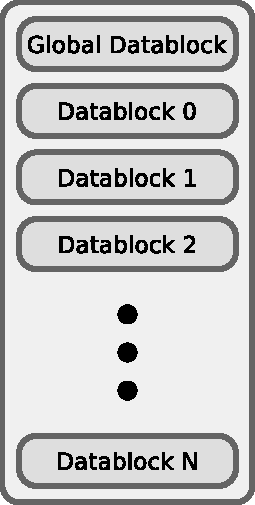
\includegraphics[scale=0.75]{./fig/structure_result_file.pdf}
  \caption{Coarse structure of a file containing simulation results.}
  \label{fig:hdfschema}
\end{figure}

The figure \ref{fig:blockschema} shows the internal structure of a single data
block. The dark blocks are at the level of individual data tensors while the
lighter grey boxes represent hdf groups. Note that not all data sets may exist
at all and that each group can have different subsets. For example if you never
computed observables, then this entire block is missing. The wavefunction data
can come from a simulation with the Fourier propagator or from the evaluation
of wavepackets on a given domain-wide grid.

\begin{figure}
  \centering
  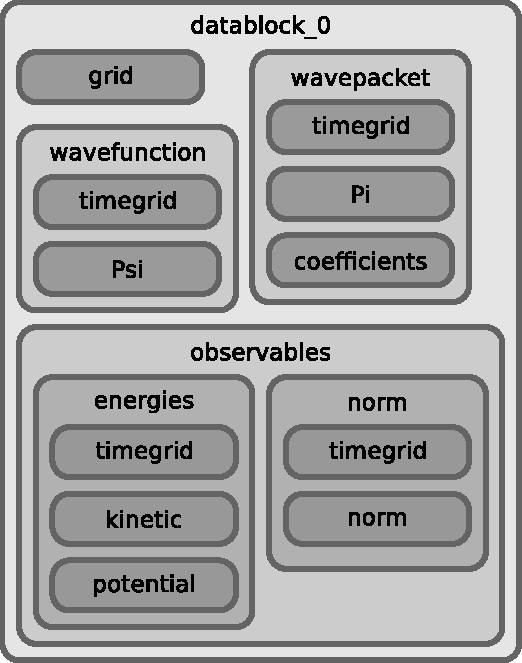
\includegraphics[scale=0.75]{./fig/structure_datablock.pdf}
  \caption{Possible structure of a single data block. Not all data does always exist.}
  \label{fig:blockschema}
\end{figure}

\subsection{Saving data at times and timesteps}

Storing simulation data can happen in various different ways. For example you
can store data at regular time intervals. Or at a list of fixed points in time.
Both is easily possible with the tools provided by the \emph{IOManager} together
with the \emph{TimeManager}. While the \texttt{IOManager} is responsible for
saving and loading the data, the \texttt{TimeManager} is used for all computations
related with time, timesteps and so on, for example to convert a list of times
into a list of timesteps or checking if a given time is is within the simulated
time range etc.

The two parameters \verb|write_nth| and \verb|save_at| are used to configure the
way you wish to save data. While the first is used to specify the details of saving
at regular time intervals, the second one provides the means to specify a list
of points in time when saving should take place. A few examples on saving at regular
intervals.

\begin{verbatim}
  # Save data at each timestep
  write_nth = 1

  # Save data each 5th timestep
  write_nth = 5

  # Never saving data at regular intervalls
  write_nth = 0
\end{verbatim}

Please note that this scheme is rigid in the sense that if for example the timestep
corresponding to the end of the simulation is not an integer multiple of the value
of this parameter then the data from the end is missing. (This should be quite obvious!)

The parameter \verb|save_at| has to be a python list containing integers
and/or floats. And there is a \emph{big difference} between the two data types
you always have to be aware of! Integers values are interpreted as \emph{timesteps}
while floats will be taken as \emph{times}. A few examples on saving at specified
times only:

\begin{verbatim}
  # Save at timestep 3, 6, 7, 13 and 19
  save_at = [3, 6, 7, 13, 19]

  # Save at the end time only
  # Assuming T = 5.34 and T is an integer multiple of dt!
  save_at = [5.34]

  # Save at a few times
  # This is usefull to compare simulation results of simulations
  # with different timestep sizes. Of course the times have to be
  # integer multiples of *all* timestep sizes in consideration!
  save_at = [3.2, 4.5, 8.7, 19.3]
\end{verbatim}

You can freely mix the two approaches and specify crazy things like
the following

\begin{verbatim}
  write_nth = 15
  save_at = [1, 2, 3, 4.5, 10, 3.2, 40, 23.45, 23.55]
\end{verbatim}

which translates to the: \emph{Save the data each 15 steps and additionally
save the data at the timesteps 1, 2, 3, 10 and 40 and save the data at the time 3.2,
23.45 and 23.55.} It is assumed the the \emph{time} is an integer multiple of the
\emph{timestep} size. (Otherwise more or less careful rounding will be applied.)
The list doesn't have to be in monotone order and duplicates will be removed as well
as values outside the interval $[0, T]$ where $T$ is the time at which the simulation
stops. A good use case for a mixed specification is for example saving a big
intervals but including the very end of the simulation:

\begin{verbatim}
  write_nth = 35
  save_at = [5.34]    # Same assumption as above
\end{verbatim}

Note that even if you disable saving data entirely be setting:

\begin{verbatim}
  write_nth = 0     # Default is 1
  save_at = []      # Default is []
\end{verbatim}

you will end up with a hdf5 file still containing the initial values as they
are at time equal 0 (before the first timestep was made).

\subsection{Retrieving the simulation parameters}

From a hdf5 file with the simulation data we can get back the parameters this
simulation used. Retrieval is trivial, the following commented interactive python
session shows the basics which can of course be used in a user script too.

\begin{verbatim}
  >>> from WaveBlocks import IOManager
  >>> iom = IOManager()                         # create an IOM instance
  >>> iom.load_file("simulation_results.hdf5")  # load the data file
  >>> sim_params = iom.get_parameters()         # request the parameters
  >>> print(sim_params)
  ====================================
  Parameters of the current simulation
  ------------------------------------
  [...]
\end{verbatim}

With only three trivial lines of code we get back all the parameters
that were used for the simulation!

\subsection{Load simulation data}

Simulation data can be loaded from a given \verb|simulation_results.hdf5| file by
an IOManager instance. You can even do this inside an interactive \texttt{ipython}
session. The API is quite trivial, all functions for loading data have their name
prefixed by \verb|load_| as for example in \verb|load_energy(...)|. Every function
for loading and saving data has a keyword argument \texttt{block} defaulting to 0
which tells the IOManager from which data block to take the requested data.
For quantities that represent time series, the load functions also provide a keyword
argument \texttt{timestep} that can be used to load data from a single timestep.
The default is \texttt{None} meaning \emph{load the data from all timesteps}.
A sample of such an interactive session could look like this:

\begin{verbatim}
  >>> from WaveBlocks import IOManager
  >>> iom = IOManager()                          # Create a new IOManager instance
  >>> iom.open_file("simulation_results.hdf5")   # And open a given hdf5 file

  >>> print(iom)
    IOManager instance with open file simulation_results.hdf5

  >>> ekin, epot = iom.load_energy()         # Load the energies from a simulation
    Requested function: load_energy          # Don't bother about the messages
    Plugin to load: IOM_plugin_energy        # concerning the plugins.

  >>> ekin.shape                             # We see the the energies are given
    (301, 1)                                 # as time series over 301 timesteps
  >>> epot.shape
    (301, 1)

  >>> tg = iom.load_energy_timegrid()        # Load the corresponding timegrid which
                                             # contains the timesteps when the data
  >>> tg.shape                               # was saved. This is important if the
    (301,)                                   # data was saved at non-regular intervalls.

  >>> iom.finalize()                         # Close the hdf5 file

  >>> plot(tg, ekin)                         # Plot the kinetic energy over time
\end{verbatim}

Of course all this works exactly the same inside any regular python script.
For a complete list of all the \verb|load_| functions please see the API
documentation or the docstrings.

\section{User scripts}

Consider merging this section with chapter 2.
Do an explicit example walk through somewhere.

\subsection{Preparing simulations}

\begin{verbatim}
  python ConfigurationGenerator.py  <metaconfiguration.py> <configurations_dir>
\end{verbatim}


\subsection{Generating Configurations}

In detail description on how to generate valid configurations

\subsubsection{Manually}

\subsubsection{Meta-configurations}

\begin{verbatim}
- You can use any valid python statement as value
- All statements are written to a pure python code file
- You can write numbers, lists etc as plain text strings
- All that is not in string form gets evaluated *right now*
- Remember to escape python strings twice
- You can use variable references but with great care!
- The ordering of the statements in the output file is such that
  all statements can be executed w.r.t. local variables. This is
  some kind of topological sorting. Be warned, it's implemented
  using black magic and may fail now and then!

  That should be all ...
\end{verbatim}

\subsection{Running simulations}

To run a single simulation, use the \texttt{Main.py} script. The first command
line argument is the simulation configuration file (with an arbitrary file path).

\begin{verbatim}
  python Main.py path/to/the/simulationparameters.py
\end{verbatim}

The results will be written to the file \texttt{simulation\_results.hdf5}
in the \emph{local} directory where the script was called and \emph{not}
where the configuration file was loaded from.

To run a bunch of simulations, use the script called \texttt{Batch.py}. It
has three command line parameters and all are optional with sensible defaults.
The first specifies the \emph{batch configuration} that will be used. The second
is a directory path pointing to the directory where the configuration files
are located. All python files within that directory (excluding recursive descent)
will be treated as simulation configurations. The directory path default to
\texttt{./configurations/}. Last but not least the third argument specifies the
directory path where the simulation results (numerical data, plots etc) will be
placed after the simulation finished. This defaults to \texttt{./results/}
with one subdirectory for each simulation configuration. A call looks like:

\begin{verbatim}
  python Batch.py batchconfiguration.py configurations_dir results_dir
\end{verbatim}

This is all you need to know to be able to run simulations.



\subsection{Computing additional data}

Only compute/store what comes out directly from the time propagation
(Or what would be much more difficult to computer afterwards)

Compute all other data in a separate step after the simulation finished
Example: Norms, energies etc

\subsection{Evaluating data}

\subsection{Plot data}

Call plot scripts which load the simulation data from a file and plot the values.



\chapter{The \texttt{WaveBlocks} library}

\section{Available blocks}

See the API documentation.


\chapter{Extending \texttt{WaveBlocks}}

In this chapter we describe the steps to extend the \texttt{WaveBlocks}
code base with respect to various central aspects. The most important aspect
is probably the possibility to add new potentials of whatever kind. The other
topics include the question on how to save more data and what it takes to
implement new simulation algorithms.

\section{Structure of potential definitions}

Performing a simulation with a new potential that is not (yet) part of the
\texttt{PotentialLibrary} is not difficult. All potentials are specified
as a python dict. An simple example of a potential definition could look like:

\begin{verbatim}
  quadratic = {}
  quadratic["potential"] = "1/2 * sigma * x**2"
  quadratic["defaults"] = {"sigma":"1/2"}
\end{verbatim}

We see that this is nothing else than a python dict (here assigned to the
variable \texttt{quadratic}). This dict must have a key \texttt{potential}
and the corresponding value is the analytic potential formula. This formula
must contain the variable \texttt{x} which is the position space variable.
It may optionally have an arbitrary number of parameters, here for example
the \texttt{sigma}.

The dict may have a further key called \texttt{defaults} whose value is
another dict containing default values for the parameters. These values
are used if you do not specify a value for a parameter in the simulation
configuration file. You may omit the defaults here, then you always have
to provide a value in the simulation configuration. Values given in the
simulation configuration always precede default values.

The analytic potential formula is given as a string. This string is parsed
by the \texttt{sympify} function of Sympy. You can use many of the usual
mathematical operations and functions, for example (fractional) powers
(\texttt{**}), roots (\texttt{sqrt()}), trigonometric and hyperbolic functions
and their inverse functions (but remember, it's \texttt{atan} and not \texttt{arctan} etc)
and also some constants like \texttt{pi}. Please refer to the Sympy manual
for a more thorough description of \texttt{sympify}. The most important point is
to make sure that the formula finally yields a scalar expression in $x$.

\newpage
A more complicated potential could be given by the following python code:

\begin{verbatim}
  delta_gap = {}
  delta_gap["potential"] = [["1/2 * tanh(x)", "delta"         ],
                            ["delta",         "-1/2 * tanh(x)"]]
\end{verbatim}

This potential has two energy levels and is given by a $2 \times 2$ matrix.
The matrix is constructed as two nested python lists. Each entry is a single
string as above. Note also that this potential does not specify a default
for \texttt{delta}, you have to assign a scalar float value to a variable
called \texttt{delta} in the simulation configuration. You may specify potentials
with as many energy levels as you like.

A final word on the strings representing formulae and parameter values: any string
that \emph{only} consists of a numerical constant my be replaced by a float. But
be careful with divisions, in python 2.x, \texttt{1/2} is \texttt{0}!

\section{Adding new potentials}

After we have seen the general structure of a potential definition in the last
section, let's now look at how to add and use a new potential. For new potentials
you have basically two options. Either place the potential definition in the
\texttt{PotentialLibrary.py} file. Make sure your variable name (for example
\texttt{delta\_gap}) is unique. If you decide to go this way, you can use
the new potential by referring to it in the simulation configuration as:

\begin{verbatim}
  potential = "delta_gap"
\end{verbatim}

The other option is to place the \emph{whole} potential definition inside the
simulation configuration file. Then this would look like:

\begin{verbatim}
  potential = {}
  potential["potential"] = [["1/2 * tanh(x)", "delta"         ],
                            ["delta",         "-1/2 * tanh(x)"]]
\end{verbatim}

This time you must name the dict \texttt{potential} because that's the
variable name where the \texttt{ParameterProvider} looks for a potential.
For the first time it might be confusing that the dict as well as its main
key both bear the name \texttt{potential} but this is correct. Of course you
can specify default values here too, but probably it has no real use case.

As a small side note, here is an example of a custom potential when we create
the configurations by the \texttt{ConfigurationGenerator}. (This is only a small
excerpt of a metaconfiguration file.)

\begin{python}
  # A custom potential without a default for "alpha"
  GP["potential"] = {}
  GP["potential[\"potential\"]"] = "\"cosh(alpha*x)\""

  # Different values for "alpha" in each simulation
  LP["alpha"] = [ 0.1*i for i in range(1,5) ]
\end{python}

Please note the escaped quotes, it's essential to do this correct here.



\section{Compute and store more data}

IOM and IOM Plugins, how to teach the IOM to store more/other data.

\section{New propagation algorithms}

Implementing the \texttt{SimulationLoop} and \texttt{Propagator} interfaces



\chapter{Software architecture}

Some comments for developers

How to achieve things that are more complicated than whats
described in chapter 5

\section{Interfaces}

\section{Class hierarchies}

\end{document}
